\documentclass[article]{ajs}

%%%%%%%%%%%%%%%%%%%%%%%%%%%%%%
%% declarations for jss.cls %%%%%%%%%%%%%%%%%%%%%%%%%%%%%%%%%%%%%%%%%%
%%%%%%%%%%%%%%%%%%%%%%%%%%%%%%
 
\usepackage{etoolbox}
\usepackage{amsmath}
\usepackage{graphicx}
\graphicspath{{images/}}
 
 
%% almost as usual
\author{Matthias Medl\,\orcidlink{0000-0002-3354-4579}\\ Institute of Statistics \\ BOKU University \\ Vienna \And 
        Dianne Cook\,\orcidlink{0000-0002-3813-7155}\\ Econometrics and Business Statistics \\ Monash University \\ Melbourne \And
        Ursula Laa\,\orcidlink{0000-0002-0249-6439}\\ Institute of Statistics \\ BOKU University \\ Vienna}
%% \AND can be used instead of \And and starts a new line
\title{LIONFISH: an expLoratory Interactive tOol for dyNamic visualization and identiFicatIon multidimenSional mecHanisms}

%% for pretty printing and a nice hypersummary also set:
\Plainauthor{Matthias Medl, Dianne Cook, Ursula Laa} %% comma-separated
\Plaintitle{LIONFISH} %% without formatting
\Shorttitle{LIONFISH} %% a short title (if necessary)

%% an abstract and keywords
\Abstract{
Lorem ipsum Lorem ipsum Lorem ipsum Lorem ipsum Lorem ipsum Lorem ipsum
Lorem ipsum Lorem ipsum Lorem ipsum Lorem ipsum Lorem ipsum Lorem ipsum
Lorem ipsum Lorem ipsum Lorem ipsum Lorem ipsum Lorem ipsum Lorem ipsum
Lorem ipsum Lorem ipsum Lorem ipsum Lorem ipsum Lorem ipsum Lorem ipsum
Lorem ipsum Lorem ipsum Lorem ipsum Lorem ipsum Lorem ipsum Lorem ipsum
Lorem ipsum Lorem ipsum Lorem ipsum Lorem ipsum Lorem ipsum Lorem ipsum
Lorem ipsum Lorem ipsum Lorem ipsum Lorem ipsum Lorem ipsum Lorem ipsum
Lorem ipsum Lorem ipsum Lorem ipsum Lorem ipsum Lorem ipsum Lorem ipsum
}
\Keywords{interactive graphics, tourr, exploratory data analysis, \proglang{R}, \proglang{python}}
\Plainkeywords{keywords, comma-separated, non-capitalized,, R} %% without formatting
%% at least one keyword must be supplied

%% publication information
%% NOTE: Typically, this can be left commented and will be filled out by the technical editor
%% \Volume{50}
%% \Issue{9}
%% \Month{June}
%% \Year{2012}
%% \Submitdate{2012-06-04}
%% \Acceptdate{2012-06-04}
%% \setcounter{page}{1}
\Pages{1--xx}

%% The address of (at least) one author should be given
%% in the following format:
\Address{
  Matthias Medl\\
  Institute of Statistics\\
  BOKU University Vienna\\
  E-mail: \email{matthias.medl@boku.ac.at}\\
}
%% It is also possible to add a telephone and fax number
%% before the e-mail in the following format:
%% Telephone: +43/512/507-7103
%% Fax: +43/512/507-2851

%% for those who use Sweave please include the following line (with % symbols):
%% need no \usepackage{Sweave.sty}

%% end of declarations %%%%%%%%%%%%%%%%%%%%%%%%%%%%%%%%%%%%%%%%%%%%%%%


\begin{document}

\section{Introduction}

Clustering algorithms are often used to find a smaller number of observations (the cluster means) that adequately summarize a much larger number of observations. For market segmentation, clustering can allow partitioning of observations into a small number of groups, by incorporating associations between the variables. Market segmentation supports targeted approaches to different groups of customers based on common traits.  It provides a data-driven solution to partitioning customer data. \cite{leisch2018market} provides an extensive overview of using clustering for market segmentation. 

A difference between clustering analysis and partitioning is typically the nature of the data. With cluster analysis, we usually envision data that contains separated clusters, and a successful clustering result is one that divides the data based on these gaps. With partitioning, it is usual that there are no gaps in the data, but it is still useful to partition the data. Figure \ref{kmeans-partition} illustrates how the $k$-means algorithm would partition a 2D data set into four groups depending on the correlation between the two variables.  When the correlation is high, the partitioning will be along the combination of variables that produces the highest variance. With lower correlation, it will segment the bottom and top, and divide the middle into two parts in the opposite direction. When there is no association, the partitioning is radial like a windmill.

\begin{figure*}[h]
\centerline{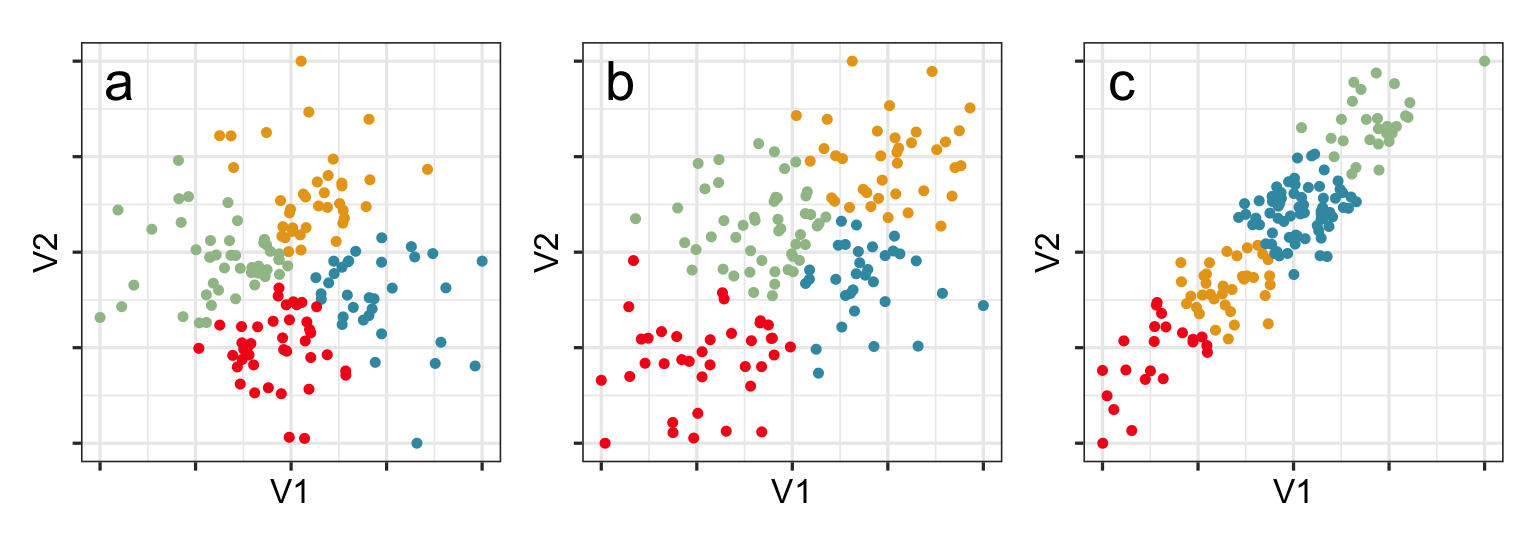
\includegraphics[width=1\textwidth]{images/intro1.png}}
\caption{Examples of how $k$-means partitions 2D data with different association structure. If the correlation is high (c), the partitioning happens along the primary direction of the association.}
\label{kmeans-partition}
\end{figure*}

One can see that the data is perfectly divided into four parts. However, if one were to plot the two variables individually, this would not be obvious. Figure \ref{kmeans-histogram} shows histograms of the two variables, V1, V2, with the colour matching the four partitions. From the histograms, we can see some differences in the partitions for the four different association structures, but they are all overlapping. The distinct border between the partitions can only be seen from the scatterplots of both variables. 

\begin{figure*}[ht]
\centerline{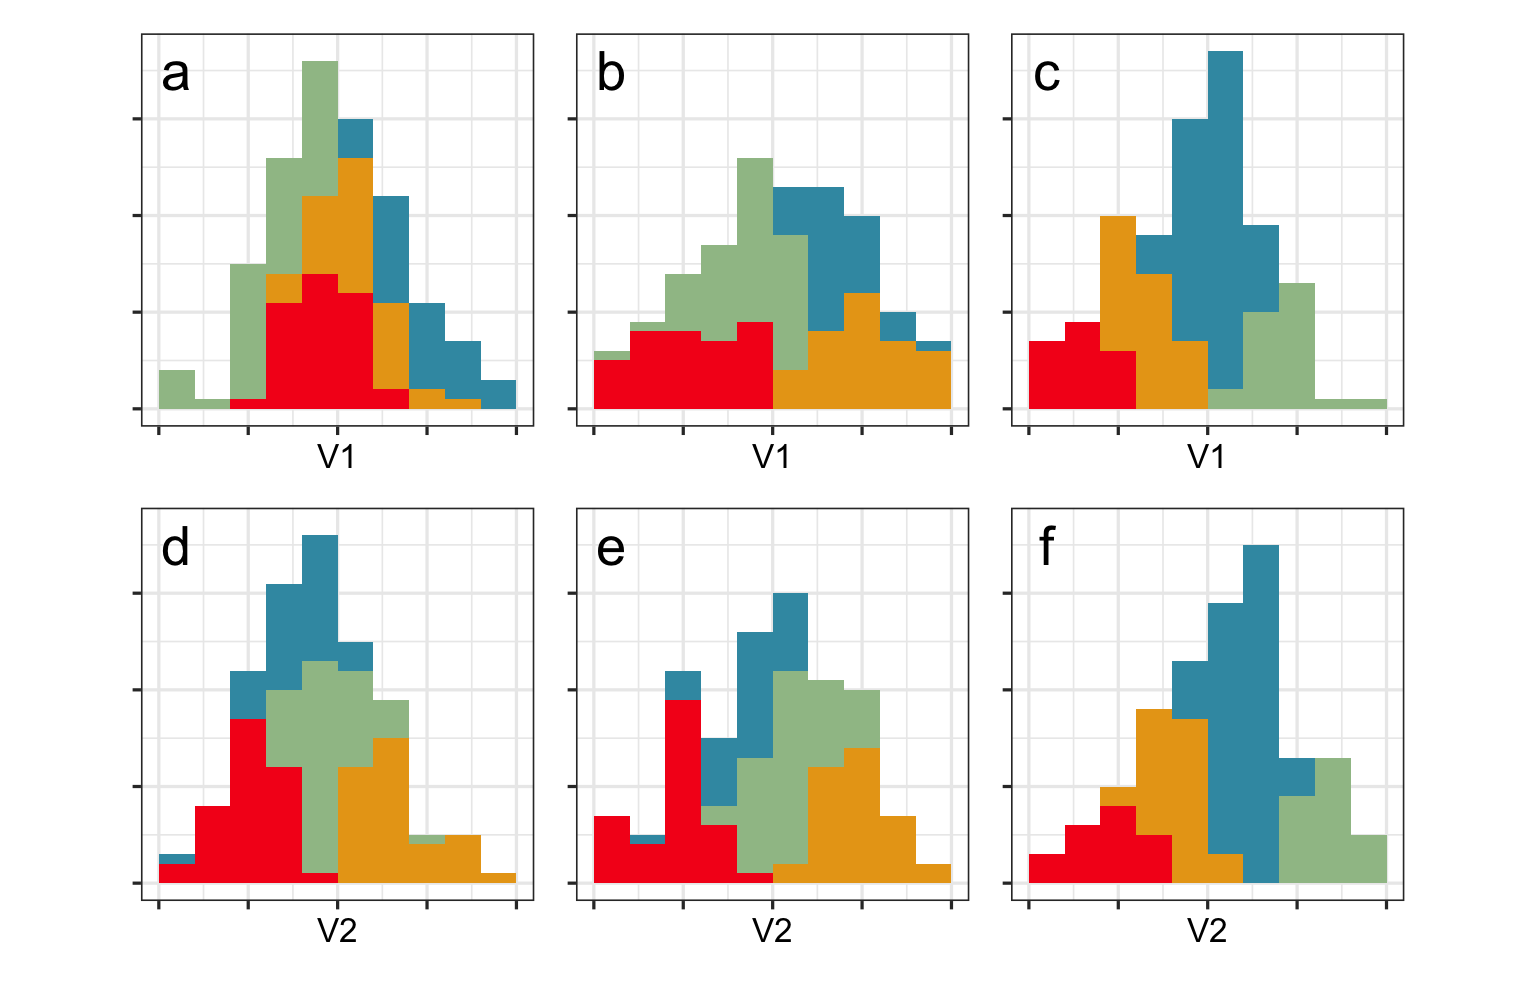
\includegraphics[width=1\textwidth]{images/intro2.png}}
\caption{The four $k$-means partitions plotted as histograms of the individual variables. While differences between groups can be seen, the clear separation cannot. This is important for understanding why high-dimensional visualisation methods are useful for summarising partitioning results.}
\label{kmeans-histogram}
\end{figure*}

When there are more than two variables, histograms of the individual variables are commonly used to display the partitioning results. This means that the analyst likely cannot understand how the partitioning divides the data. All that they can observe is roughly how the individual variables relate to the partition, which is useful but inadequate. Here is where using tour methods to view high dimensions can be helpful. A tour (\cite{Asimov1985-xr}, and see \cite{lee2022}) can be used to show scatterplots of combinations of variables and thus provide views like that in Figure \ref{kmeans-partition} where distinct differences between partitions can be observed. High dimensions are still tricky, and a combination of animations of the linear combinations, and interactive control \citep{cook_manual_1997, laa2023new} over the combinations is important. A scatterplot of a combination of variables can be considered to be a projection of the data, and thus like a shadow of a 3D object, some aspects of the data (object) can be obscured. Using slices of the projected data \citep{Laa2020} can be a useful addition to projections. This paper illustrates how to do this to better understand partitioning results for multivariate data.

%\begin{itemize} \itemsep 0in
%\item Background to clustering analysis
%\item Visualising clusters, including tours
%\item Difference between clustering and partitioning
%\item How do you know whether the results are useful
%\end{itemize}

This paper is organised as follows. Section \ref{interface} describes the software interface. The user workflow is explained in \ref{workflow}.  The methods are illustrated in Section \ref{applications} using Austrian and Australian tourism data provided in \cite{leisch2018market}. Sections \ref{discussion} and \ref{conclusion} discuss the limitations and potential future developments.

\section{Interactive interface for partitioning}~\label{interface}

The aim of this work is to build an interface that allows for an interactive exploration of partitioning solutions of multivariate data. The interface should enable

\begin{itemize}
\item visualizing a clustering solution with different tour methods, including manual changes to the viewing direction (manual tour)
\item brushing of (groups of) points for manual refinement of the cluster solution (spin-and-brush capabilities)
\item additional linked displays for comprehensive exploration of the solution
\item ability to update the displays based on user selections
\end{itemize}

While tour animations are best obtained within R using the tourr package~\citep{tourr}, it does not enable the interactivity required for example for a manual tour~\citep{laa2023new}. Interactive graphics are available when using Javascript, as implemented in the detourr package \citep{RJ-2023-052}. This allows to replay a recorded tour path with interactive graphics, and can also be linked with additional displays, but lacks capabilities for manual tours.

To integrate user interactions with the capabilities of the tourr package an active communication with the interface is required. For example, we may wish to explore the local neighbourhood of a projection selected by the user with a local tour animation provided by tourr, or we may want to optimize a guided tour path using groups identified via brushing.
Our solution is using Python for high-performance interactivity, through the packages \texttt{TKinter} \citep{lundh1999introduction}, \texttt{CustomTKinter} \citep{schimansky24}, and \texttt{matplotlib} \citep{Hunter:2007}, with integration to the tourr package \citep{tourr} via \texttt{reticulate} \citep{reticulate}, a framework that facilitates seamless interoperability between Python and R.
\textcolor{red}{also rpy2?}

%At the core of the \texttt{pytourr} package is a graphical user interface (GUI) designed to display multiple linked visualizations concurrently. Users can interact with one of the plots, for example, by subselecting specific data points, and the other linked plots will dynamically update to reflect these modifications. This interconnected functionality allows for efficient and immediate analysis of high-dimensional datasets without necessitating extensive coding, thereby streamlining the exploratory data analysis process.

The interface was implemented in \texttt{pytourr} and offers a variety of linked interactive plot types, providing users with the flexibility to visualize their data from multiple perspectives. The ability to navigate through various projections of the displayed tours directly within a graphical user interface (GUI) enables users to explore different aspects of the dataset. Furthermore, users can initiate new tours directly from the interface. The GUI also supports interactive variable selection, allowing users to specify which subset of variables should be visualized in the plots. Once users have identified interesting views or settings, \texttt{pytourr} allows them to save the displayed projections, subsets, and plots. This functionality ensures that analysis states can be preserved for further examination or reporting, making the package particularly useful for iterative analysis where findings may need to be revisited or shared with collaborators.

With its high level of interactivity, performance, and ease of use, \texttt{pytourr} streamlines the exploration of complex datasets, offering a powerful tool for researchers working with high-dimensional data.


\subsection{Overview of the graphical user interface (GUI)}

The \texttt{pytourr} GUI can be launched using the function \texttt{interactive\textunderscore tour()}. At a minimum, the user needs to provide both the dataset and the instructions for constructing the desired plots. The dataset must be supplied as a \texttt{data.table}, while the plotting instructions should be passed as a list containing the named elements \texttt{type} and \texttt{obj}. The \texttt{type} element specifies the type of display to generate, such as \texttt{scatter} for a scatterplot or \texttt{2d\textunderscore tour} for a 2-dimensional tour. The \texttt{obj} element further defines the properties of the chosen display. For example, to create a 2-dimensional tour, the user must provide a \texttt{tour\textunderscore history} object, which can be generated using the \texttt{tourr} package. For a scatterplot, the user needs to provide a vector of strings specifying the names of the features to be displayed. The user can optionally specify the feature names, the arrangement of the plots, predefined subsets of the data (e.g., cluster solutions), custom names for these subsets, the number of available subsets, and the size of each plot.

The GUI is divided into two main sections: a sidebar on the left, which contains a comprehensive set of interactive controls, and the display area on the right, where the selected plots are shown (see Figure \ref{fig:GUI_overview}).

At the top of the sidebar, users can select and deselect features using checkboxes (Figure \ref{fig:GUI_overview}C), controlling which features are displayed in the plots. Below this, each subset has its own checkbox to designate the active subset (Figure \ref{fig:GUI_overview}D). When data points are manually selected in the plots, they will be assigned to the active subset and colored accordingly. For scatterplots, data points can be selected by encircling them directly on the plot while holding down the left mouse button. For barplots, clicking on a specific bar selects the data represented by that bar. The colored boxes next to the subset names indicate the assigned colors for the data points. Clicking on these boxes adjusts the transparency of the points, which is helpful for highlighting and comparing subsets. Subsets can also be renamed using the provided text boxes. The \texttt{Reset original selection} button allows users to revert the subset selections to their initial state.

The frame selection interface (Figure \ref{fig:GUI_overview}E) displays the frames of the currently shown tours and enables users to jump between frames of the tour objects. Below this, users can save and load projections and subsets using the respective buttons (Figure \ref{fig:GUI_overview}F). New tours can be started using the current settings via the interface at the bottom (Figure \ref{fig:GUI_overview}G), and users can select different metrics for some plot types e.g. heatmaps (Figure \ref{fig:GUI_overview}H).

\begin{figure}[h!]
    \centering
    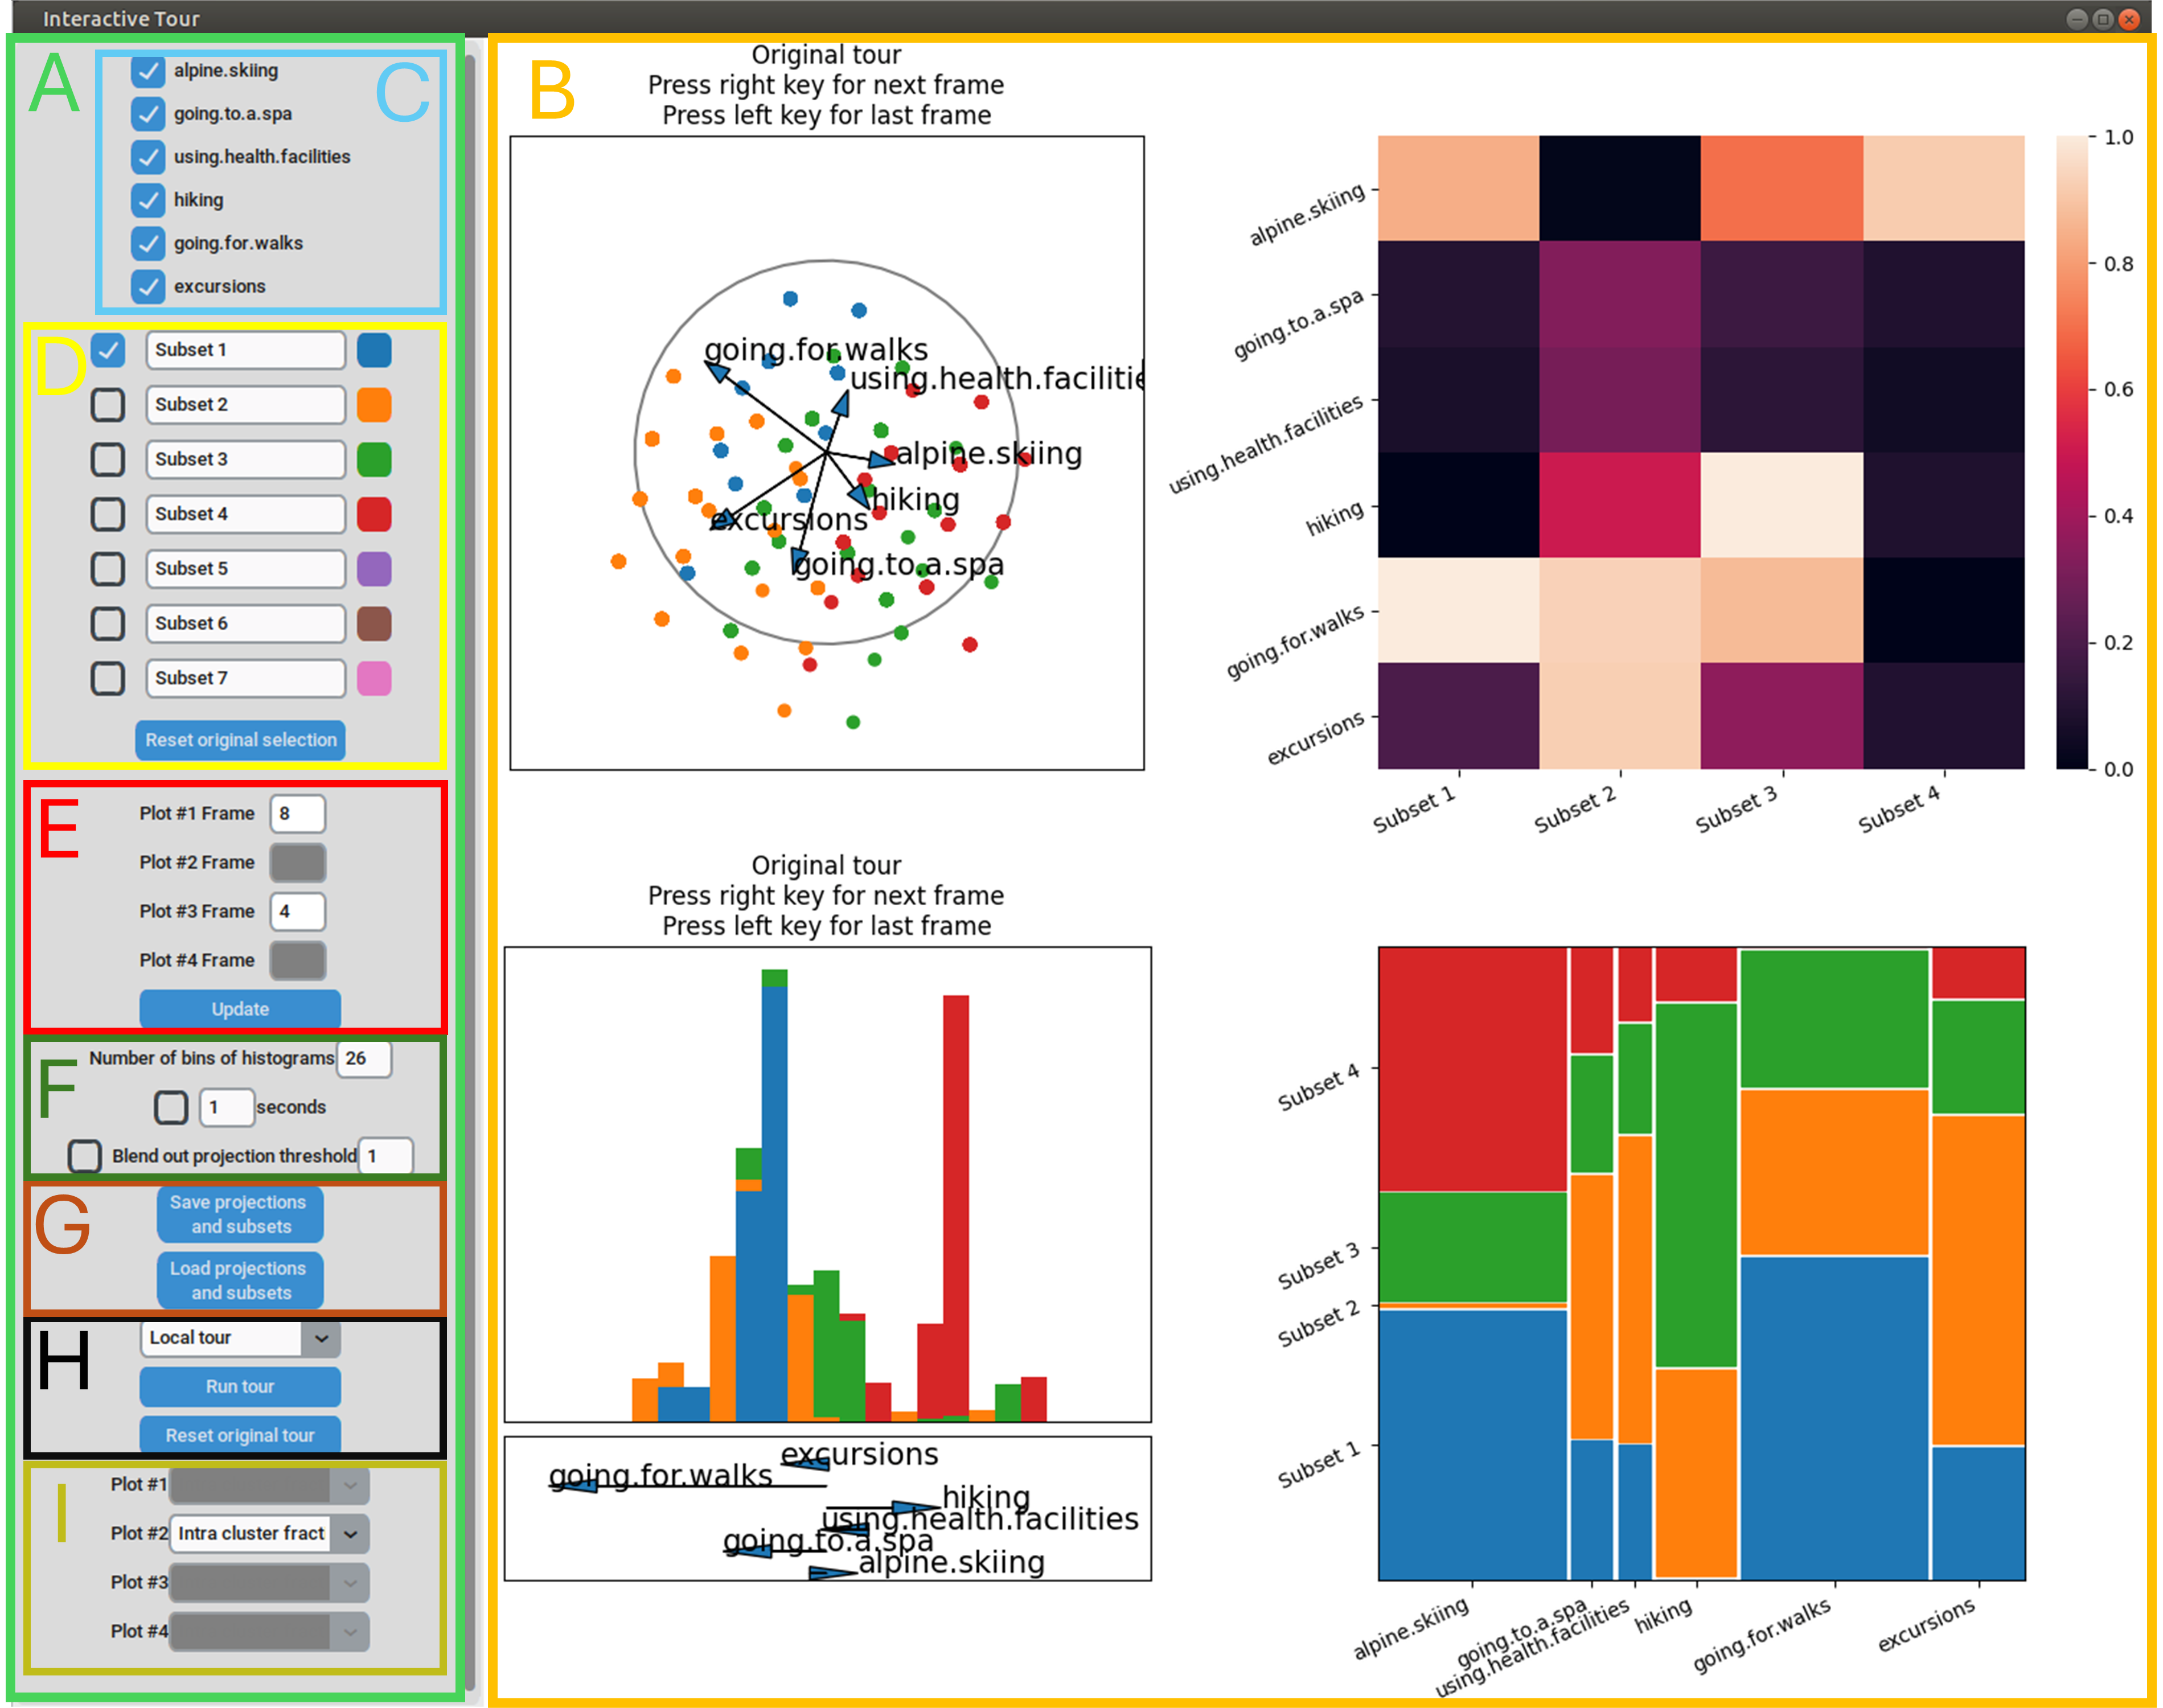
\includegraphics[width=1\textwidth]{GUI_overview.png}
    \caption{Overview of the GUI. A: Sidebar controls; B: Display area;  C: Feature selection checkboxes; D: Subset selection with color indicators; E: Frame selection interface; F: Save and load buttons; G: Interface for starting new tours; H: Metric selection interface.}
    \label{fig:GUI_overview}
\end{figure}


One can move through the projections of a tour by pressing the arrow keys or by specifying the index of the projection the be displayed and pressing the \texttt{Update frames} button. Users can animate the tours by toggling the \texttt{Animate} checkbox and specifying a time interval, so that the displays automatically move to the next projections after the specified time interval.

The \texttt{Save projections and subsets} button can be used to save the current state of the analysis. These states can be recovered by using pressing the \texttt{Load projections and subsets} button. Additionally, users can initiate new tours of various directly from the sidebar.


\subsection{R/Python interface}

The majority of \texttt{pytourr} was written in Python, while the R side of the package handles setting up the Python environment within the interactive interface is being run, launching the interactive tour, and generating new tours when initiated through the interface. To incorporate the functionality of the \texttt{tourr} package without translating large portions of its code from R to Python, the \texttt{reticulate} package was used. This approach allows \texttt{pytourr} to automatically benefit from updates to \texttt{tourr}.

However, to reduce inefficiencies caused by cross-language communication and to simplify debugging, \texttt{tourr} functions were only accessed when necessary. Core functionalities, such as performing data transformations using projections, were implemented directly in Python. These transformations are based on well-established mathematical principles and are straightforward to replicate, ensuring they remain stable and efficient.

\subsection{Structure of the Python code}

The central component of the Python code is the \texttt{customTKinter} class \texttt{InteractiveTourInterface}. This class centrally stores attributes related to all plots, such as the dataset, sub-selections, feature selections, and other shared information. Plot-specific data is organized in dictionaries (the Python equivalent of named lists in R), including the display type, construction instructions, tour projections (only in case of tour displays), color schemes for the displayed data, and, where applicable, the selector and manual projection manipulation classes.

The selector classes handle the behavior when users manually select data points to move them to the active subset. After a selection is made, the selector class updates the centrally stored sub-selection attribute and ensures all other displays reflect these changes. The manual projection manipulation classes construct the arrows representing the projection axes in the displays and manage the manual adjustment of projections, and thus enable manual tours. Users can right-click and drag the arrowheads to modify the projections, after which the class orthonormalizes the projection axes and updates both the projection and the transformed data accordingly.

\subsection{Bit blit}

The implementation of bit blitting was crucial to ensuring fast plot updates and providing a smooth user experience. With bit blit, the static elements of the display, such as the outer frames of the plots, are stored as a background image. When a plot is manipulated, only the affected plot is updated, and within that, only the interactive elements, such as the data points and projection axes in a 2-dimensional tour, are rendered on top of the background image.

In practice, this means that the background, without the interactive elements, must be captured either during initialization or after major updates. The entire plot is first rendered without the interactive elements, the background is then saved, and finally, the plot is redrawn with the interactive elements blended in. Since this process is relatively slow, full updates are only triggered during initialization or after significant changes, such as modifications to the set of active features.

\section{Workflow with the pytourr package}~\label{workflow}

Before launching the pytourr interface the user should have performed a partitioning of their choice, and provide the initial clustering solution used by the interface. We launch the interface to explore and potentially refine this solution.

\subsection{Variable selection}

A first step may look into what variables are important for the cluster solution. The interface provides different capabilities that support variable selection. First, a 2D tour view can be used to understand the sensitivity of the grouping to individual variables, in particular when using the manual tour to remove one variable at a time. This is in particular useful when the starting view was obtained through a projection pursuit guided tour~\citep{CBCH94} that optimized for the separation between the labeled groups~\citep{lckl2005}.

In our applications we are considering market segmentation analysis on binary variables. For this setting we have developed a heatmap display that we have found to be particularly useful in variable selection. The idea is to understand differences in the binary ratings between clusters, where we use different normalizations to better explore the data. For \(c_{ij}\) the count (number of true values in the binary variable) in the \(i\)-th cluster and \(j\)-th variable, we define


\[
\text{Overall count fraction}\ f_{ij} = \frac{c_{ij}}{n}
\]
with normalization to the total number of observations $n$ for a general overview,

\[
\text{Cluster count fraction}\  f_{ij} = \frac{c_{ij}}{n_{i}}
\]
showing the counts relative to the cluster's size \(n_i\), to see the fraction of observations in cluster $i$ for which variable $j$ was true, and


\[
\text{Variable count fraction}\ f_{ij} = \frac{c_{ij}}{c_{j}}
\]
to see how the true values for variable $j$ are distributed across the different clusters relative, with normalization to the overall count of that feature \(c_j = \sum_i c_{ij}\).
 
\textcolor{red}{different symbol for each? indicat on the index value somehow?}

\subsection{Subset selection}

The spin-and-brush approach suggests to cluster data manually when using a tour: we run a tour animation, stop when we see a group of points that are different from the rest of the distribution, brush them, and then continue. Different projections will enable the separation of different groups, and for well-separated clusters we will be able to recover a full cluster solutions in this manner.

A similar approach can be used to refine a partitioning solution. This is in particular useful to integrate prior knowledge or business interests in a given cluster solution. In the interface we can keep the provided clustering, but separate out new subsets via manual selection, for example after we found a group of particular interest via a manual tour.

\subsection{Reproducibility}

Ensuring the reproducibility of data analysis is a fundamental principle in scientific research. It allows others to verify the validity of the findings and is key to the integrity of the scientific process. Reproducibility not only builds trust in the research outcomes but also enables the scientific community to build upon existing work. When analyses can be replicated, it can be validated whether the conclusions drawn from the data are robust and not dependent on the specific conditions or idiosyncrasies of the original analyst. Moreover, reproducible research can serve as a foundational building block for subsequent studies, fostering incremental advancements in knowledge.

One challenge in the context of interactive data analysis is that not all steps of the analysis are precisely documented in the form of code, especially when using graphical user interfaces (GUIs) where user-driven interactions might not leave a traceable history. This lack of documentation can hinder the ability of others to reproduce the analysis or to understand how specific results were obtained. To mitigate this challenge, it is essential to implement mechanisms that allow users to easily save and share intermediate snapshots of their analyses.

One measure to combat this is to make saving intermediate snapshots of the analysis easy and accessible. Specifically, the \texttt{Save projections and subsets} button enables users to take snapshots of their analysis, including visual representations, selected data, and parameter settings. Upon pressing this button, a file browser is triggered, allowing users to specify the destination for saving these snapshots. Each save operation generates multiple files:


\begin{itemize}
    \item A \texttt{.png} file containing the currently displayed graphics,
    \item \texttt{.csv} files that capture the feature and subset selection as well as projections of the tours displayed at the time of the snapshot,
    \item two \texttt{.pkl} files that contain state variables of the GUI, allowing for complete recovery of the snapshot.
\end{itemize}

These files provide dual utility. First, they allow users to fully recover the state of the analysis within the GUI. This can be achieved either by using the \texttt{Load projections and subsets} button, or by launching a new GUI instance with the \texttt{load\_interactive\_tour()} function. The latter approach, using \texttt{load\_interactive\_tour()}, has the added flexibility of only requiring the original dataset and the directory containing the saved files. This function also allows users to modify display settings, such as adjusting the size of the interactive plots or changing the arrangement of the display grid. In contrast, when loading the saved state directly from within the GUI, it is crucial that the active session was initiated with the same dataset and plot objects that were present at the time of saving. This ensures that the analysis environment is accurately replicated.

Second, the saved \texttt{.csv} files provide a way to inspect and further analyze the data outside of the original interface. This opens up opportunities for deeper analysis and extensions of the work.

This level of interactivity and documentation is crucial for reproducibility, as it ensures that even exploratory, interactive data analysis can be retraced and validated by others. Ultimately, these features facilitate a reproducible workflow that balances the flexibility of interactive exploration with the rigor of reproducible research.


\section{Applications}~\label{applications}

The Austrian Vacation Activities \cite{dolnicar2003winter} and the Australian Vacation Activities \cite{cliff2009formative} datasets are used to illustrate the methods.

\subsection{Austrian Vacation Activities dataset}

The Austrian Vacation Activities dataset comprises responses from 2,961 adult tourists who spent their holiday in Austria during the 1997/98 season. Participants were asked to evaluate the importance of 27 different activities during their vacation. The survey categorized responses based on four levels of importance: ``totally important'', ``mostly important'', ``a bit important'', and ``not important''. For analysis, the responses were binarized: a value of 1 was assigned if the activity was rated as ``totally important'', and a value of 0 if any of the other categories were selected. The survey was conducted by the Europäisches Tourismus Institut GmbH at the University of Trier and focused exclusively on tourists who did not stay in the country's capital cities.

To gain further insight into the dataset a k-means clustering as described in \cite{leisch2018market} has been performed. Therefore, the function \texttt{stepcclust} of the R package \texttt{flexclust}\citep{flexclust} with $k=6$ and $nrep=20$ was used.

\subsubsection{Feature selection}

The original dataset contains \(p\)=27 features. Some of these features are more informative than others. We only want to keep the most informative ones. Additionally, interacting with the pytourr GUI becomes cumbersome when handling more than \textasciitilde
 15 features, making it necessary to reduce the dimensionality of the dataset. An effective and intuitive way to perform feature selection is by using the heatmap display within pytourr. 

\begin{figure}[h!]
    \centering
    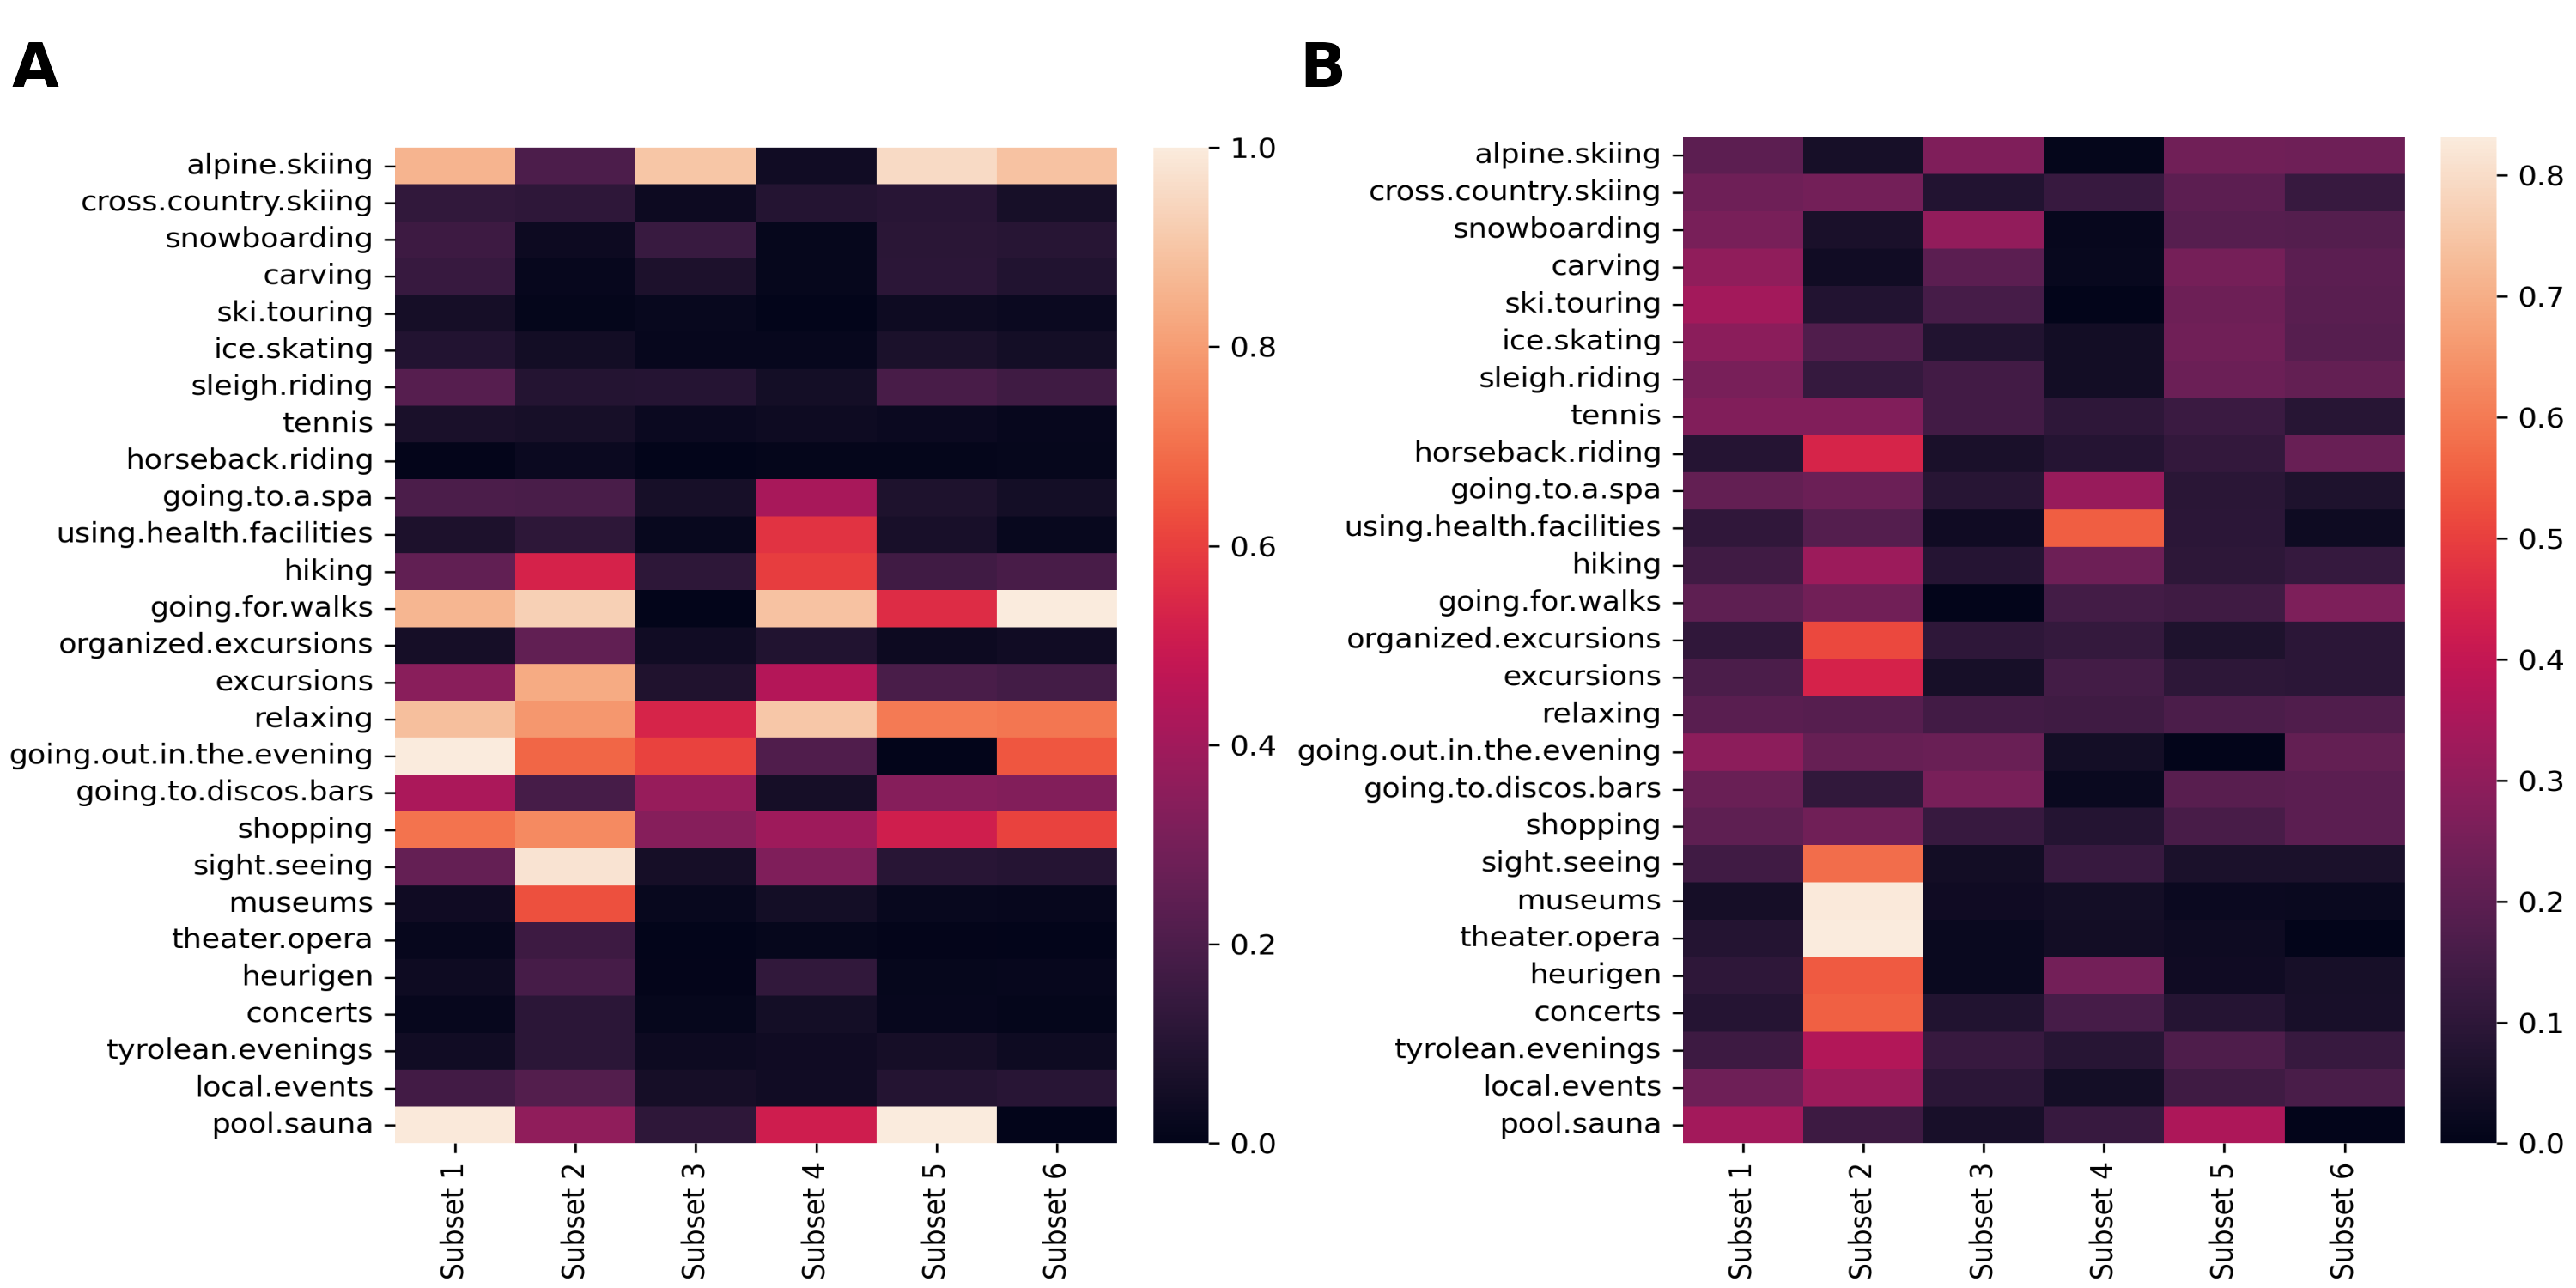
\includegraphics[width=1\textwidth]{winteractiv_heatmap.png}
    \caption{Traditional overview of clusters. Color represents  (A) the intra-cluster fraction, and (B) the intra-feature fraction, with lighter indicating higher values. From A, we can see that some activities dominate most clusters, e.g. relaxing and going for walks. Some activities are unique to clusters, e.g. skiing is a primary activity for clusters 1, 3, 5, 6. From B, we can see which activities dominate each cluster, e.g. cluster 4 tourists like going to a spa and using health activities.}
    \label{fig:winteractiv_heatmap}
\end{figure}

\textcolor{red}{It might be better to standardise these intra fractions. For A, one should divide by cluster count, and then compute activity fraction. For B, one should divide by activity count and then compute cluster fraction.} In Figure \ref{fig:winteractiv_heatmap}A, we can observe the general interests of tourists within each cluster. For instance, tourists in clusters 1, 3, 5, and 6 predominantly engaged in alpine skiing, while those in clusters 2 and 4 did not. Additionally, we see that activities such as ski touring and horseback riding were generally unpopular across all clusters.

In Figure \ref{fig:winteractiv_heatmap}B, we can determine whether tourists in a particular cluster had a strong preference for certain activities. For example, nearly all tourists who visited museums are grouped in cluster 2, and those who used health facilities are primarily attributed to cluster 4. We can also identify activities that were similarly popular across all clusters, such as relaxing.

By using the heatmap with these metrics, we can perform feature selection by removing unpopular activities and those that were consistently similar across all clusters. After performing the feature selection by unchecking the corresponding checkboxes in the GUI using this strategy, the following 12 activities remained: alpine skiing, going to a spa, using health facilities, hiking, going for walks, excursions, going out in the evening, going to discos/bars, shopping, sightseeing, museums, and pool/sauna.

We can now repeat the k-means clustering with \texttt{stepcclust} on the reduced dataset. Silhouette plots of both cluster solutions can be seen in Figure \ref{fig:silhouette_comparison}. By comparing both silhouette plots, we can see that the cluster solution with the reduced dataset results in a clustering of higher quality. Thus, we will continue with the analysis on the reduced dataset with the corresponding cluster solution. We can also see in Figure \ref{fig:silhouette_comparison}B that cluster 3 is of comparatively low quality. It is important to note that the silhouette scores were generally quite low, reflecting the lack of clearly separable clusters in the data. Consequently, there is no objectively correct or optimal solution. The primary aim of this analysis, therefore, is to gain insights into the data rather than to identify the optimal clustering configuration.

\begin{figure}[h!]
    \centering
    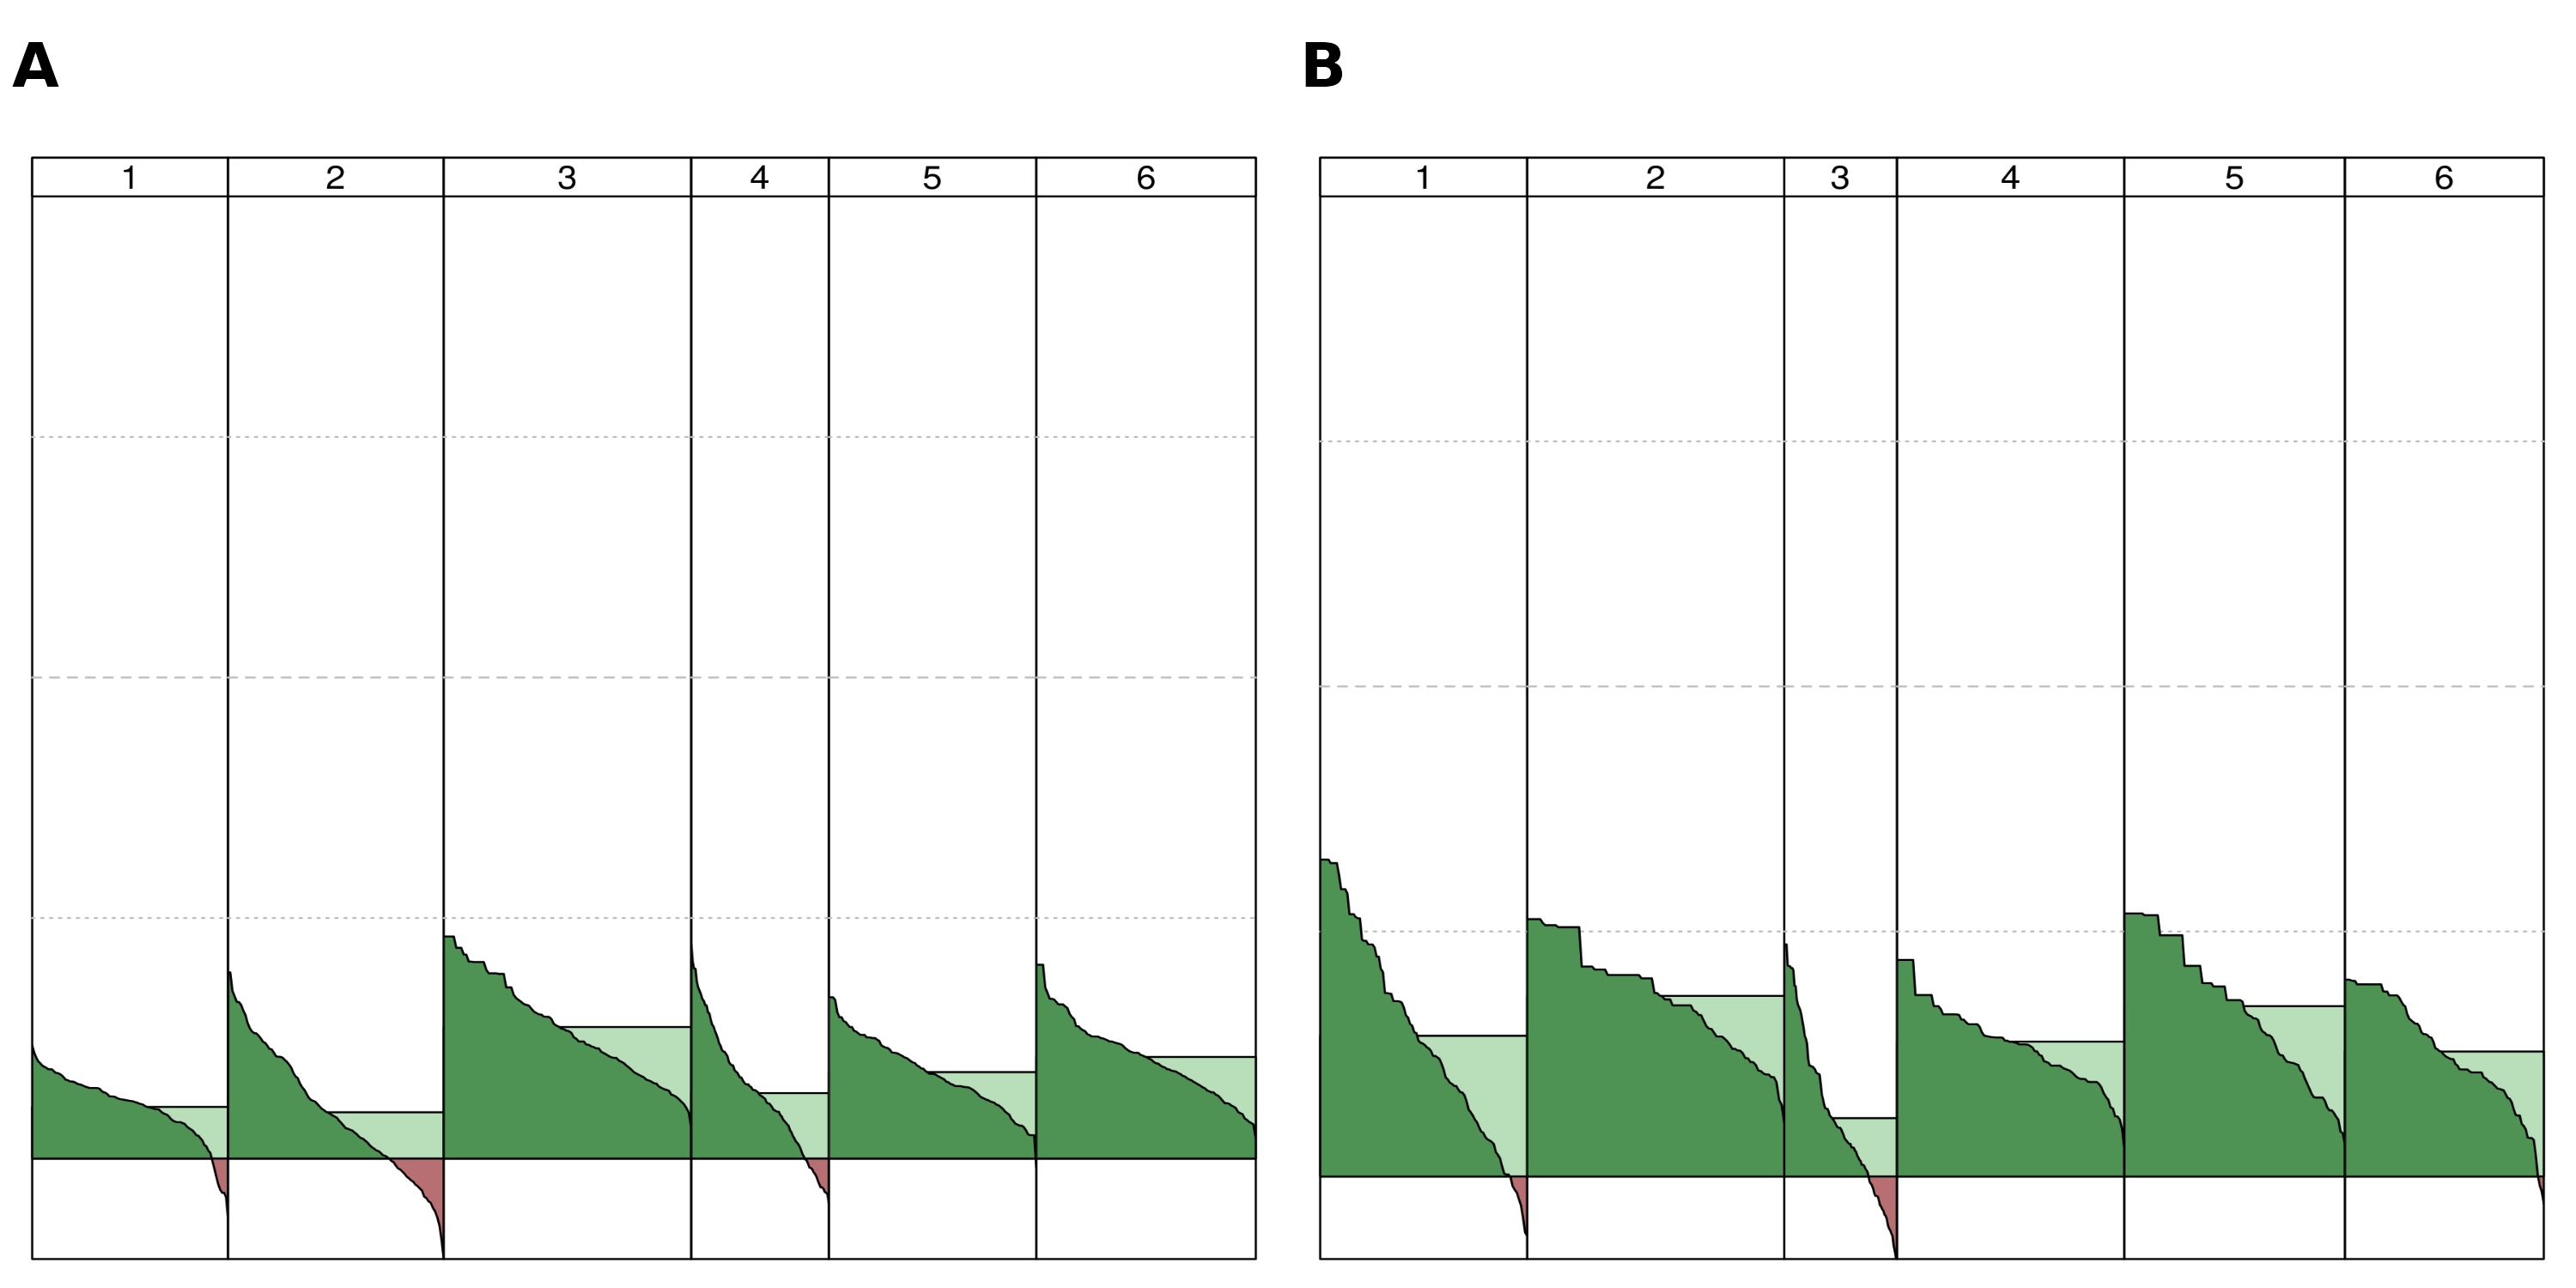
\includegraphics[width=1\textwidth]{silhouette_comparison.png}
    \caption{Comparison of silhouette plots of two k-means cluster solutions of the Austrian vacation activities dataset with k=6. (A) shows the silhouette plot of the k-means solution of the full dataset and (B) the silhouette plot of the k-means solution of the dataset after manual feature selection. We can see that the cluster solution with the reduced dataset achieved better silhouette scores and that clusters 1 and 3 contain observations with negative silhouette scores.}
    \label{fig:silhouette_comparison}
\end{figure}

We can further explore the similarities between the clusters by initializing an \texttt{interactive\_tour()} with a 2D tour based on the linear discriminant analysis (LDA) projection pursuit index. By navigating through the tour, we can observe various projections, and when a projection that separates the clusters is found, we highlight each cluster sequentially. The different highlighted clusters can be seen in Figure \ref{fig:silhouette_comparison}.

\begin{figure}[h!]
    \centering
    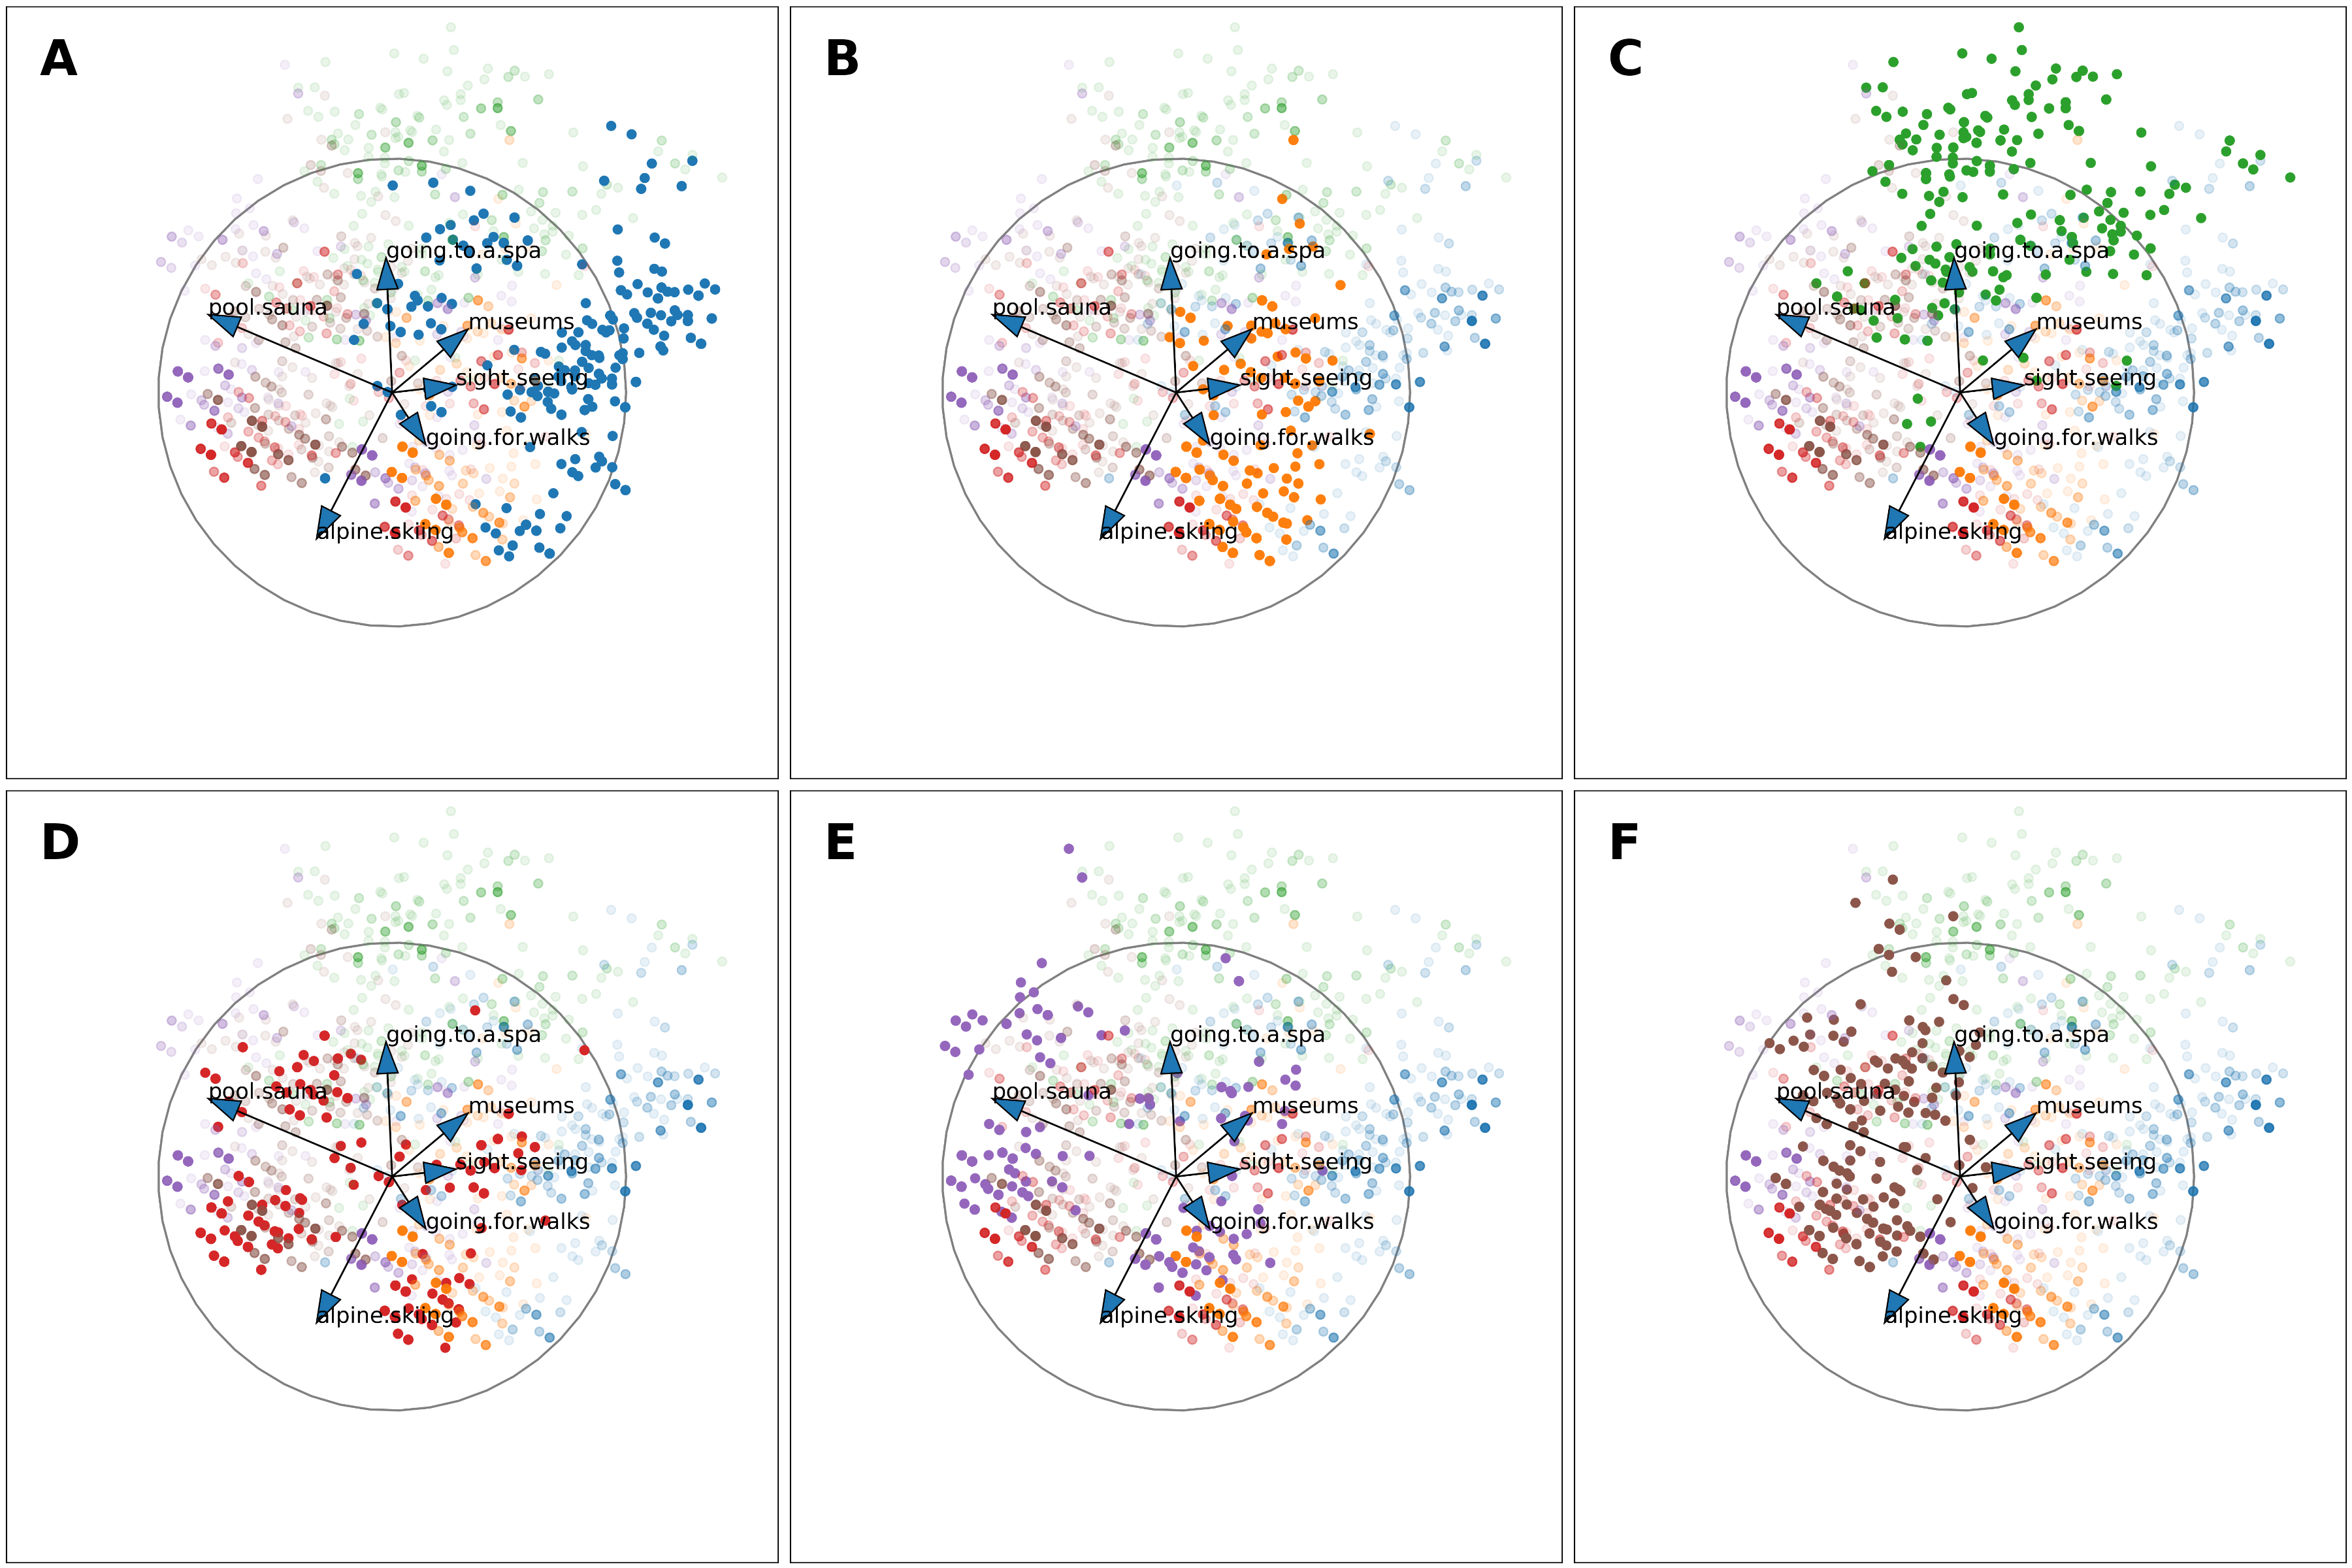
\includegraphics[width=1\textwidth]{winter_activ_cluster_highlights.png}
    \caption{Display of a projection of the Austrian vacation activities dataset with the six clusters of the k-means cluster solution highlighted in different colors. The colors indicate which clusters the highlighted observations belong to with cluster 1 being blue (A), cluster 2 being orange (B), cluster 3 being green (C), cluster 4 being red (D), cluster 5 being violet (E) and cluster 6 being brown (F). We can see that the projection separates some clusters well, however also that there is considerable overlap of clusters 4, 5 and 6}
    \label{fig:winter_activ_cluster_highlights}
\end{figure}

This process allows us to visually assess the separation and similarities between the clusters, providing insight into the structure of the dataset. By highlighting each cluster individually, we can evaluate their distinctiveness in different projections. The most influential features shown in Figure \ref{fig:winter_activ_cluster_highlights} are pool/sauna, alpine skiing, museums, and going to the spa. The projection roughly separates clusters 1 (blue), 2 (orange), and 3 (green) from each other and the other three clusters (red, violet and brown), which appear to be quite similar. 

By manually manipulating the projection axes or initiating a local tour, we can gain further insight into the similarities between the different clusters. This interactive exploration allows for a more nuanced understanding of the relationships between clusters and the influence of key features on the separation of the data.


\subsubsection{Redefining cluster assignments - learning more about museum goers}

There are several reasons why we might want to manually modify a clustering solution. One is to capture observations that do not fit well within their assigned clusters. Another reason is to explore specific features in more detail. The advantage of manual cluster selection is that it preserves most of the current clustering structure, allowing us to adjust specific parts of the solution without starting from scratch. This approach is particularly useful when we already have a cluster solution that reveals interesting patterns in the data.


In Figure \ref{fig:silhouette_comparison}, we observed that clusters 1 and 3 contained data points that did not fit well into their respective clusters. To further investigate this, we can initialize an \texttt{interactive\_tour()} with the following components:

\begin{figure}[h!]
    \centering
    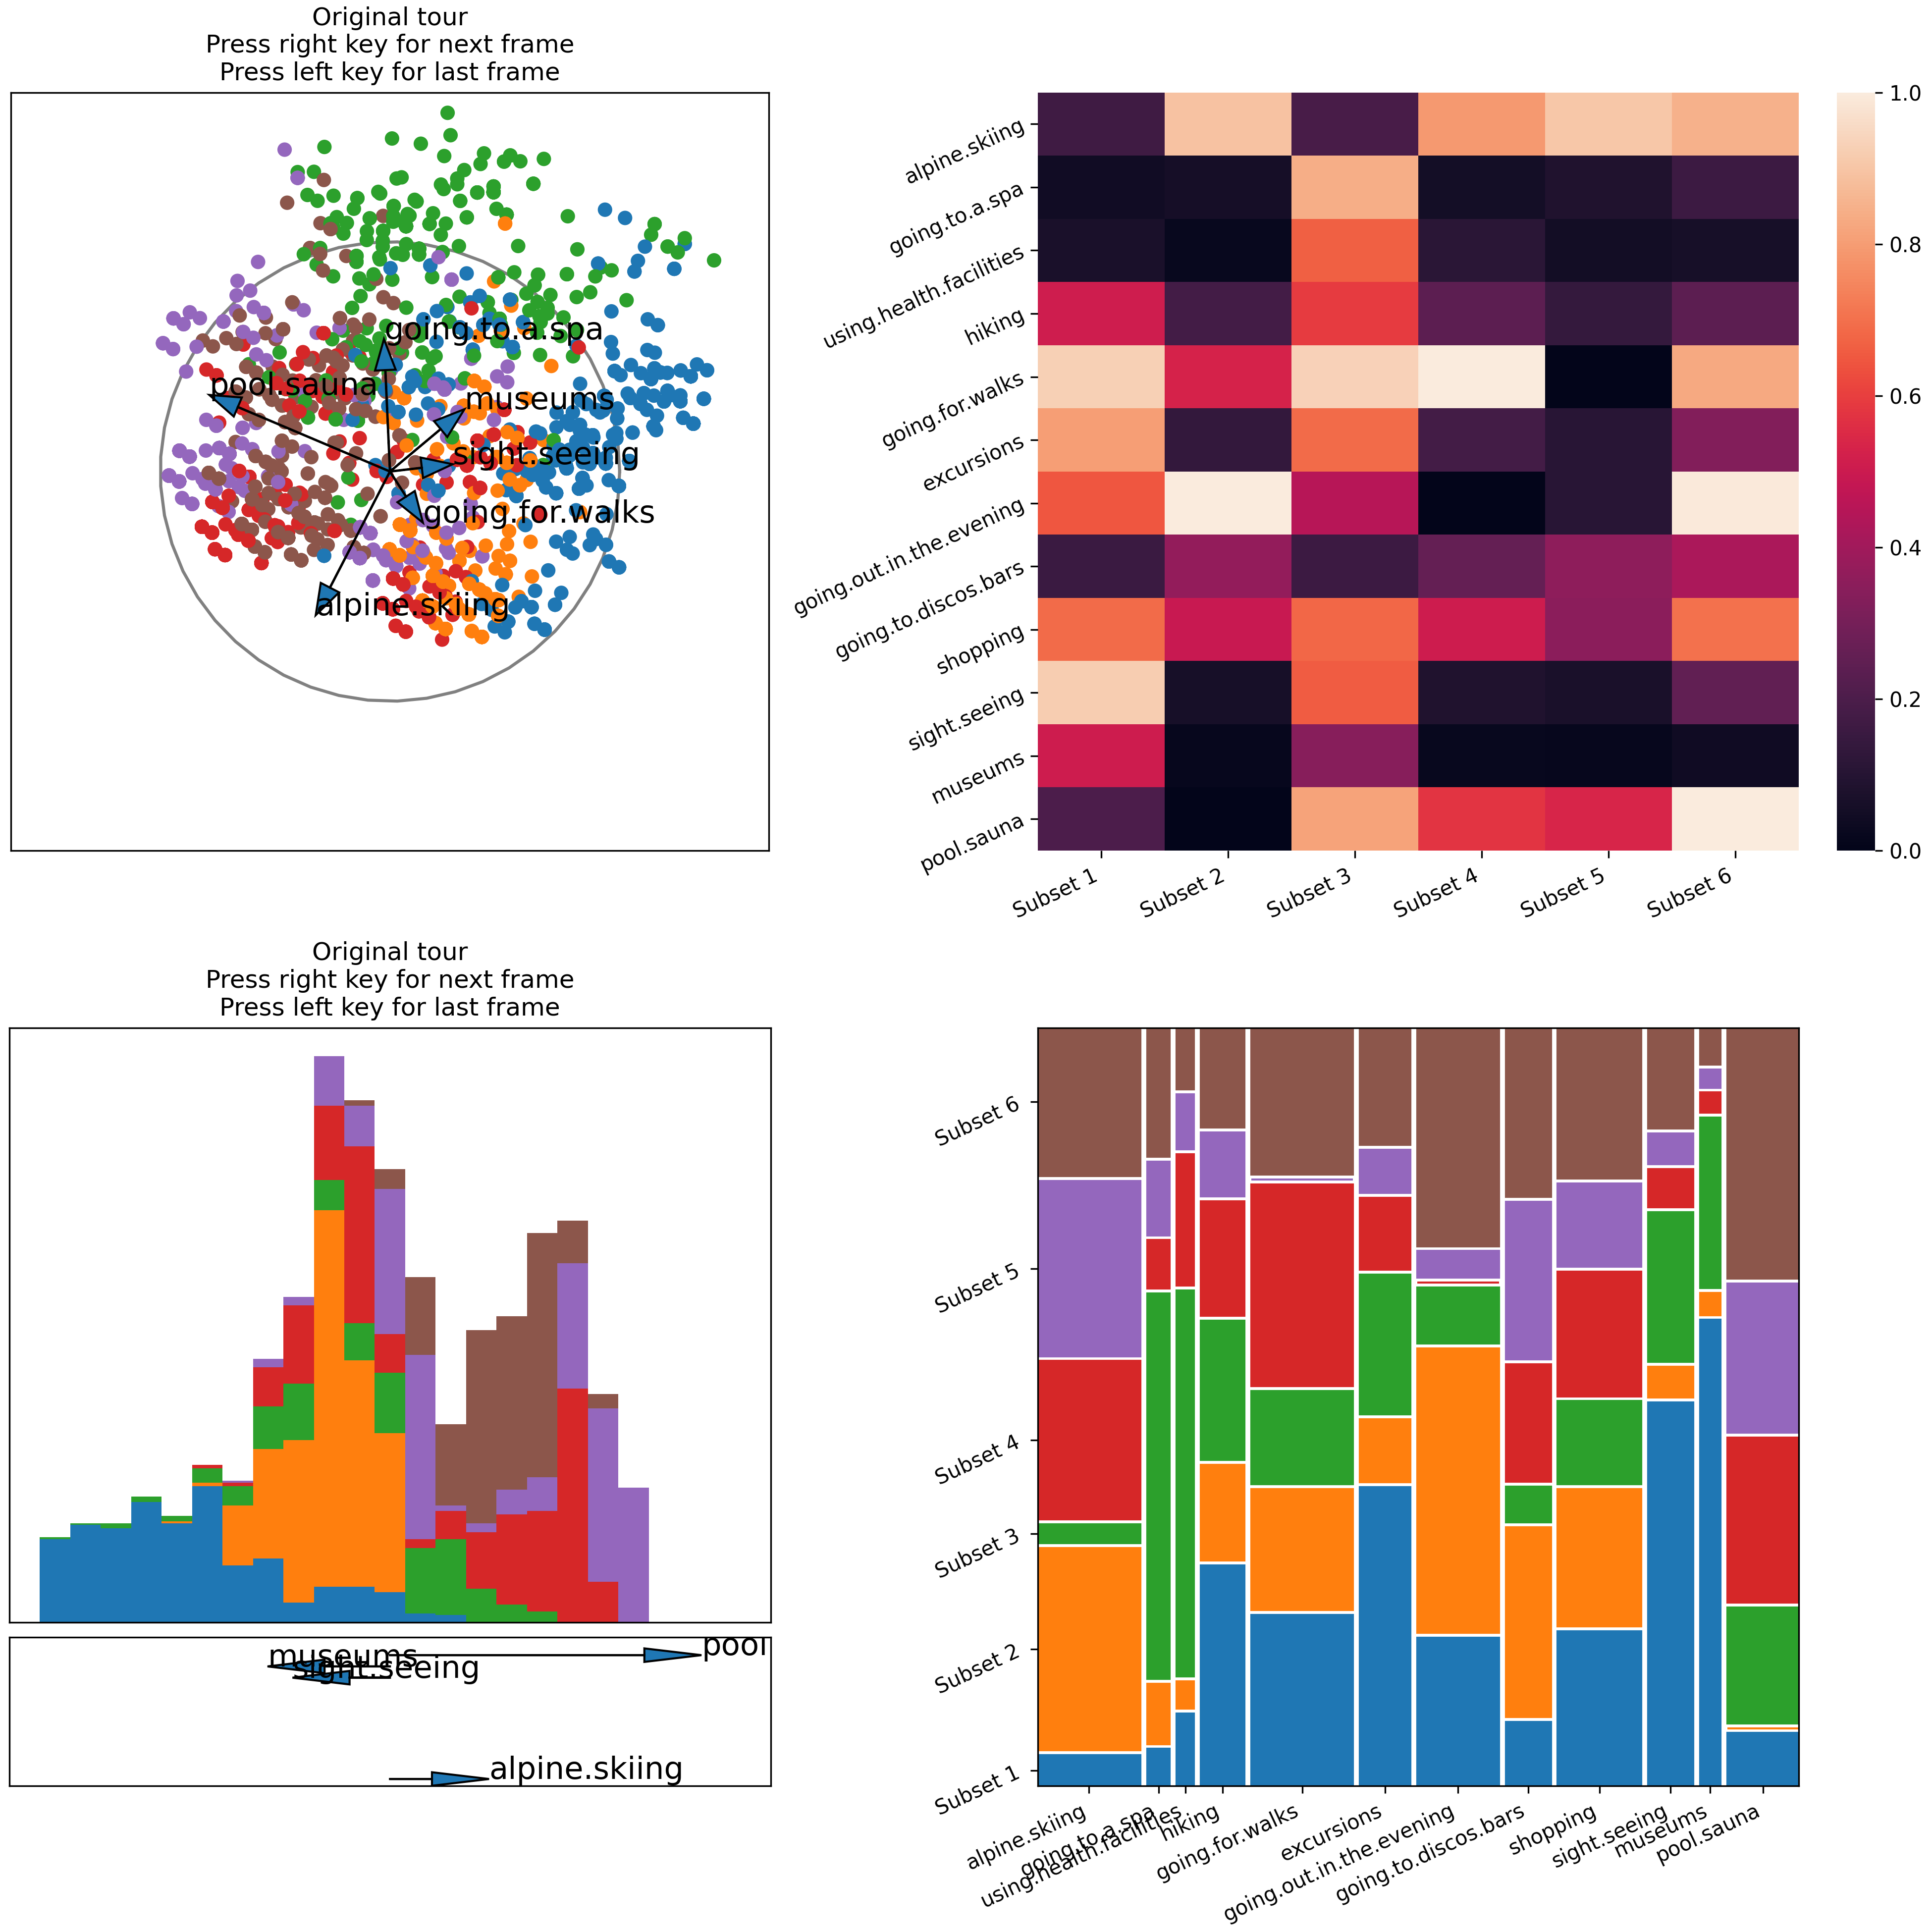
\includegraphics[width=1\textwidth]{winter_cl7_init.png}
    \caption{Interactive tour GUI loaded with multiple plots showing different aspects of the k-means solution of the Austrian vacation activities dataset. Top left: 2D tour with the linear discriminant analysis projection pursuit index. Top right: heatmap with the intra-cluster fraction. Bottom left: 1D tour with the linear discriminant analysis projection pursuit index. Bottom right: mosaic plot. Tourists in both clusters 1 and 3 didn't participate in skiing a lot, but tourists in cluster 3 were much more interested in going to the pool, spa and health facilities compared to cluster 1.}
    \label{fig:winter_cl7_init}
\end{figure}

\begin{itemize}
    \item A 2D tour using the linear discriminant analysis projection pursuit index,
    \item A heatmap showing the intra-cluster fraction,
    \item A 1D tour with the linear discriminant analysis projection pursuit index, and
    \item A mosaic plot.
\end{itemize}

This setup produces the display shown in Figure \ref{fig:winter_cl7_init}. It can also be seen that both clusters 1 and 3 contain tourists that didn't go alpine skiing and the main difference between them is that tourists in cluster 3 enjoyed going to the spa and health facilities as well as going to the pool, while the ones in cluster 1 didn't. Other than that, the clusters were mostly similar. Now we might be interested in the subset of tourists that enjoy going to museums. Therefore, we can adjust the projection axes so that these axes are elongated and point into different directions. We can see that there is indeed overlap between clusters 1 and 3, as shown in Figure \ref{fig:winter_cl7_pre}. As a next step we can reassign the overlapping section to a new cluster - cluster 7 (pink). By selecting the checkbox for subset 7 and manually selecting the region of overlap, we can form a new cluster, which is visualized in Figure \ref{fig:winter_cl7_post}.

\begin{figure}[h!]
    \centering
    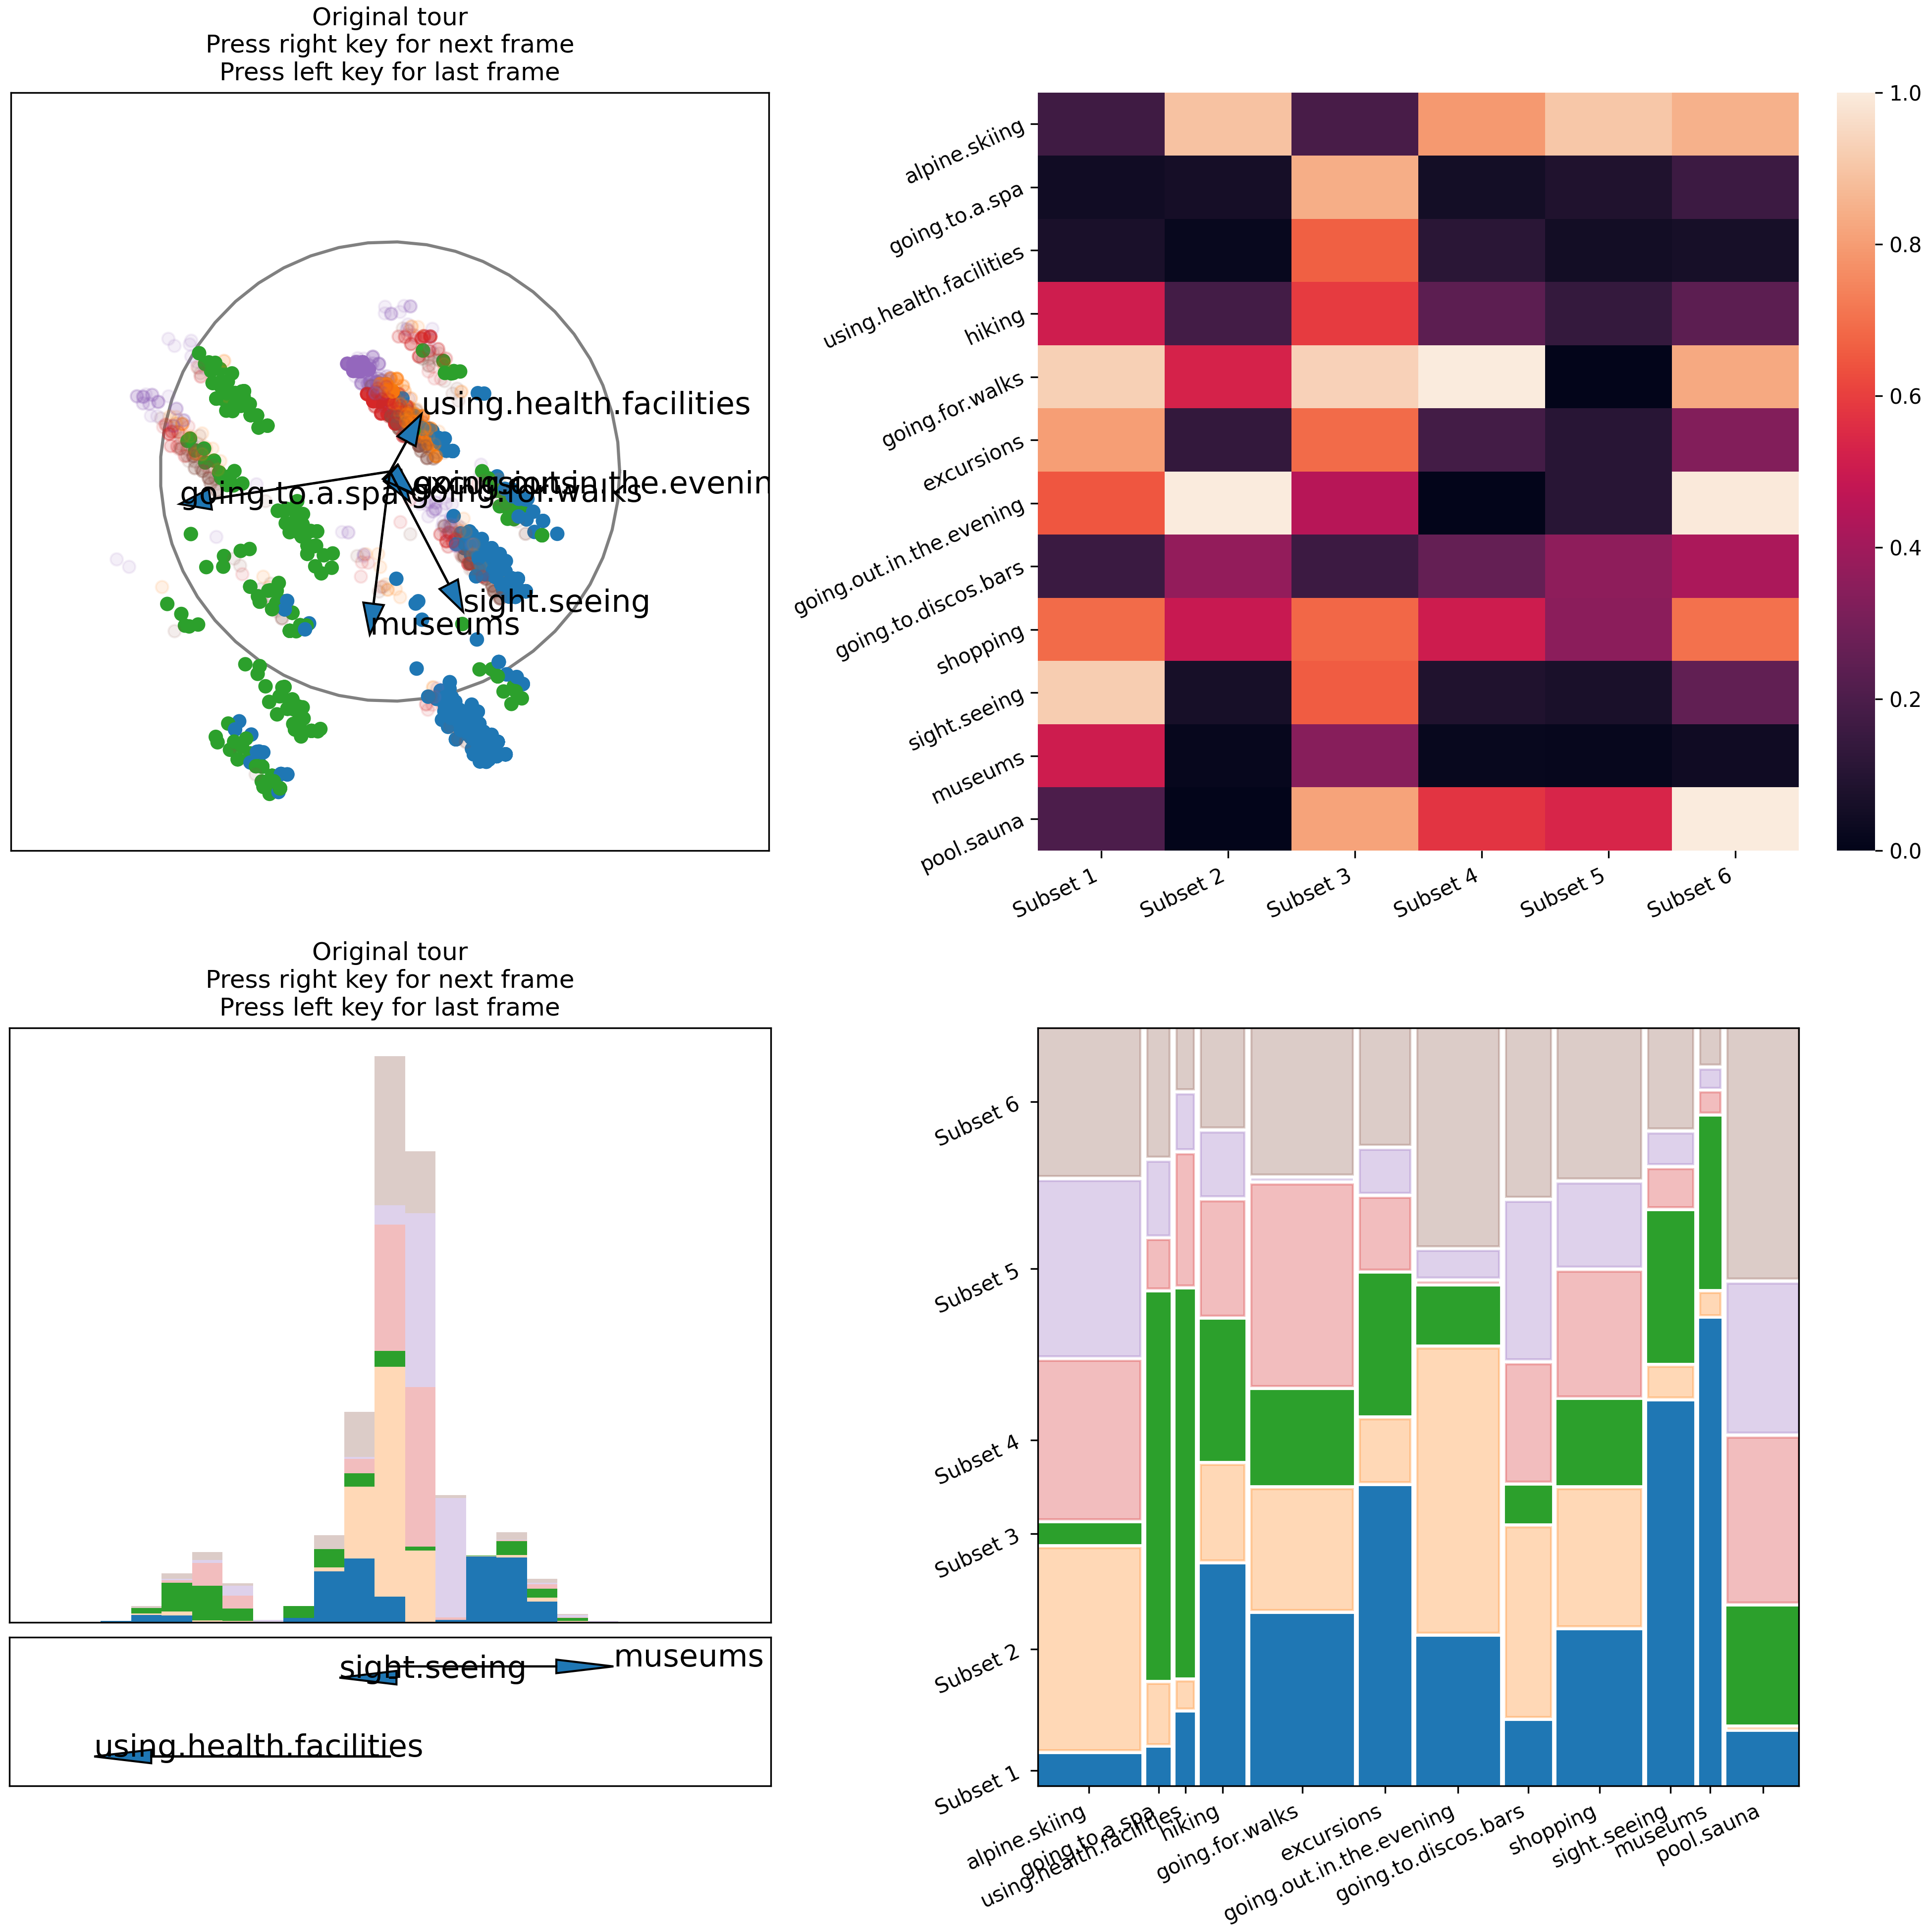
\includegraphics[width=1\textwidth]{winter_cl7_pre.png}
    \caption{Interactive tour GUI loaded with multiple plots showing different aspects of the k-means solution of the Austrian vacation activities dataset, with manually adjusted projections. Top left: 2D tour with the linear discriminant analysis projection pursuit index. Top right: heatmap with the intra-cluster fraction. Bottom left: 1D tour with the linear discriminant analysis projection pursuit index. Bottom right: mosaic plot. Changing the projection axes of ``going to a spa'', ``museums'', ``sightseeing'' and ``using health facilities'' reveals the preferences and overlap of clusters 1 and 3.}
    \label{fig:winter_cl7_pre}
\end{figure}

\begin{figure}[h!]
    \centering
    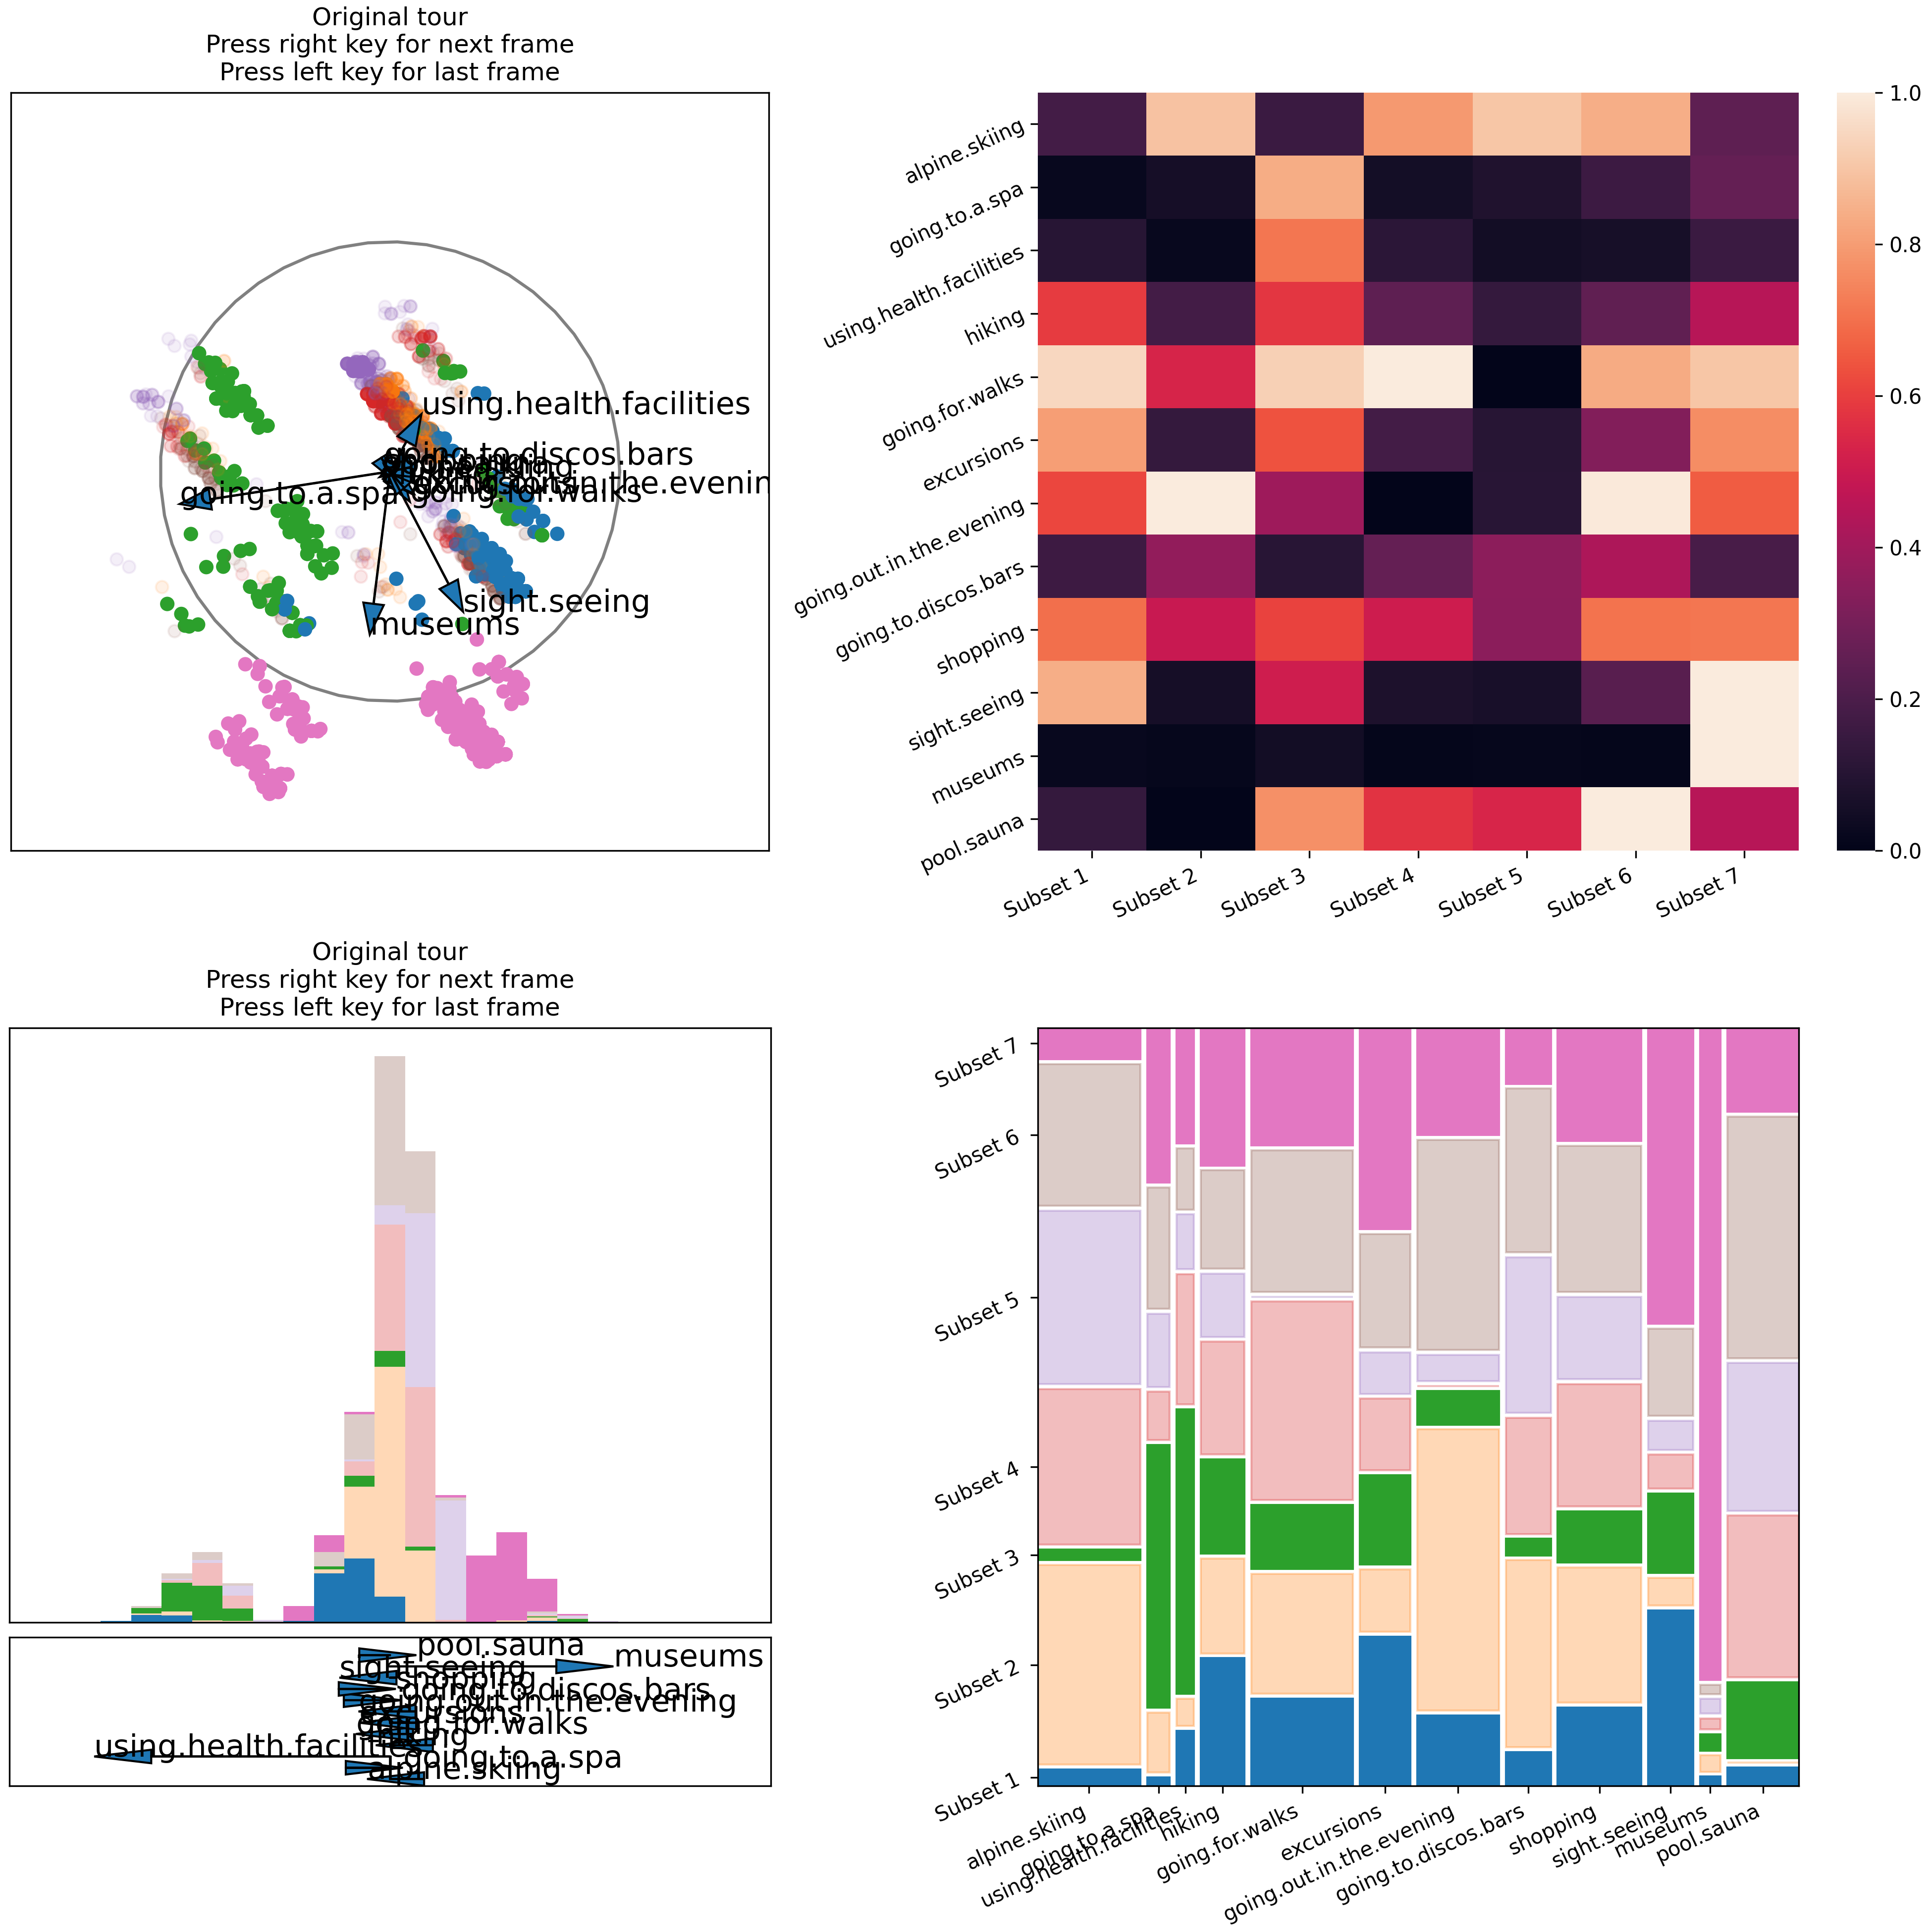
\includegraphics[width=1\textwidth]{winter_cl7_post.png}
    \caption{Interactive tour GUI loaded with multiple plots showing different aspects of the k-means solution of the Austrian vacation activities dataset, after new subsets have been selected. Top left: 2D tour with the linear discriminant analysis projection pursuit index. Top right: heatmap with the intra-cluster fraction. Bottom left: 1D tour with the linear discriminant analysis projection pursuit index. Bottom right: mosaic plot. We can see that now almost all museum goers are in the new manually selected subset 7 and what their preferences are compared to the other clusters.}
    \label{fig:winter_cl7_post}
\end{figure}


We can observe slight behavioral differences between tourists in clusters 1 and 7. Tourists in cluster 7 all enjoyed both museums and sightseeing, whereas most tourists in cluster 1 engaged in sightseeing but showed no interest in museums. Instead, participants in cluster 1 exhibited a greater preference for hiking. Despite this, tourists in both clusters generally shared similar interests. This insight could be valuable for enhancing museum marketing strategies. While clusters 1 and 7 have overlapping interests, it appears that current marketing efforts may not effectively reach tourists in cluster 1. By increasing targeted marketing at hiking trails, popular excursion destinations, and shopping centers, it may be possible to attract more interest in museums from tourists in cluster 1.

\subsection{Australian Vacation Activities dataset}

The second dataset, the Australian Vacation Activities dataset, includes responses from 1,003 adult Australians who were surveyed through a permission-based internet panel. The survey was conducted in 2007. Participants were asked whether they engaged in 44 specific vacation activities during their most recent vacation within Australia. Similar to the Austrian dataset, responses were binarized: a value of 1 indicates that the participant took part in the activity, while a value of 0 signifies they did not. Surveys where participants claimed they partook in more than 40 activities or no activity at all were removed as they are considered faulty.

\subsubsection{Feature selection}

At first, hierarchical clustering using Ward's method \citep{murtagh2014ward} and the Jaccard index was applied to the features. The resulting dendrogram is shown in Figure \ref{fig:aus_feature_clustering}. Based on this clustering, \( k = 15 \) clusters were identified, and generally, only one representative feature from each cluster was selected for further analysis. Clusters containing unpopular activities, such as ``Adventure'', which only had 42 participants, were discarded. The cluster containing popular features like ``Beach'', ``Swimming'', ``ScenicWalks'', ``Markets'', ``Sightseeing'', ``Friends'', ``Pubs'', ``BBQ'', ``Shopping'', ``Eating'', ``EatingHigh'', ``Movies'', and ``Relaxing'' was treated differently. Multiple features from this cluster were retained to preserve as much information as possible. After feature selection, the observations were reclustered using k-means with \( k = 15 \).


\begin{figure}[h!]
    \centering
    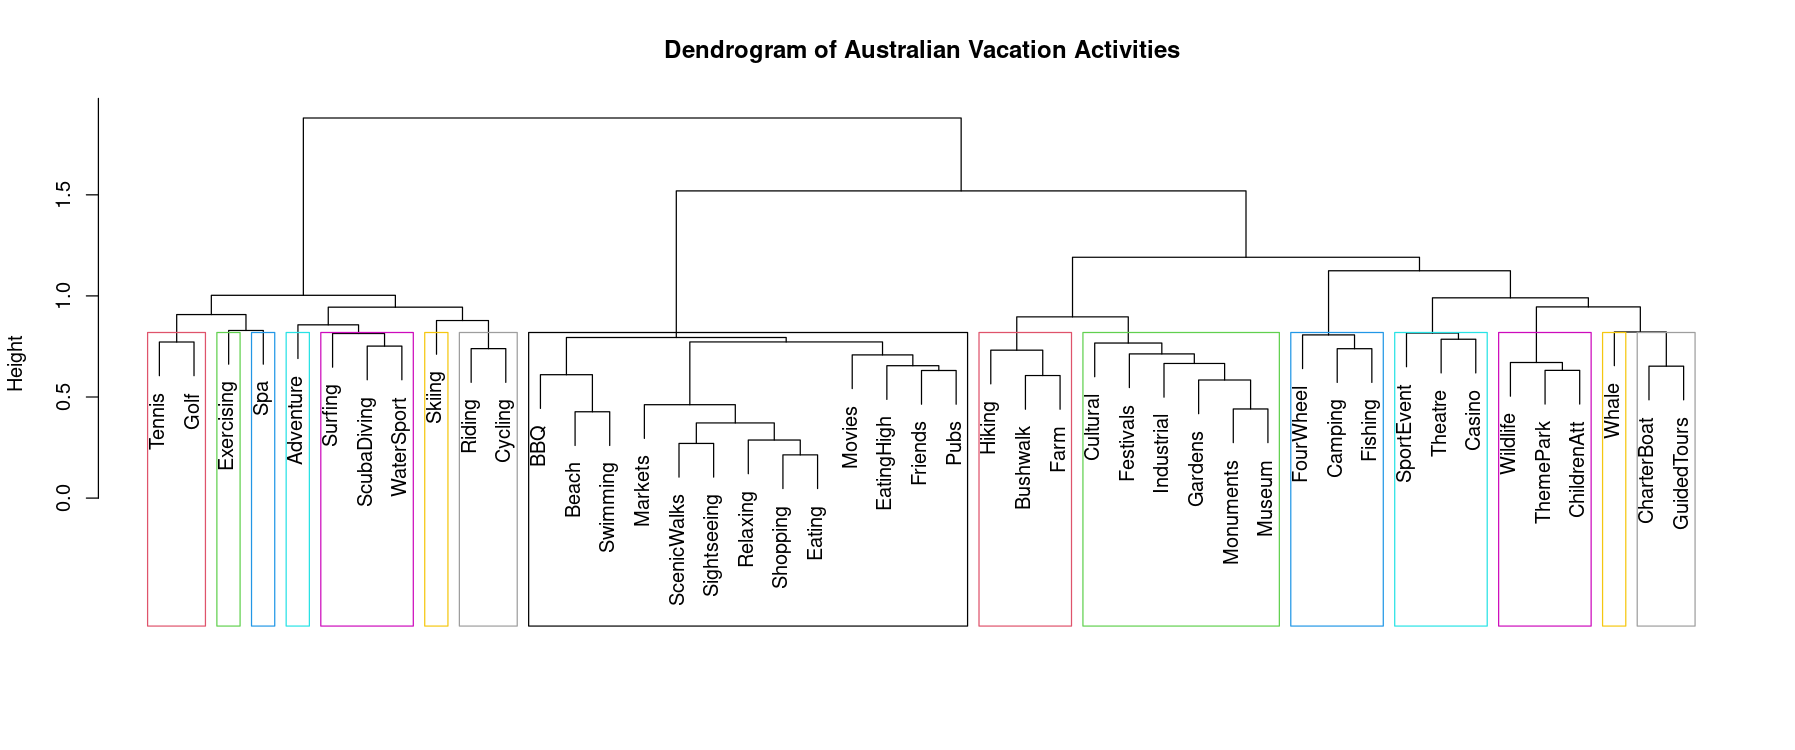
\includegraphics[width=1\textwidth]{aus_feature_clustering.png}
    \caption{Dendogram of the features of the Australian Vacation Activities dataset using Ward's method with the Jaccard index. Features which were clustered together are marked by the colored boxes. We can see, which activities had similar patterns in tourist interest.}
    \label{fig:aus_feature_clustering}
\end{figure}

\subsubsection{Segmentation of solo travellers}

In the heatmap displaying the intra-cluster fraction shown in Figure \ref{fig:aus_heatmapg}, we observe that subsets 1, 2, and 6 tend to prefer travelling alone. As a tourist agency, we might be interested in targeting solo travellers more effectively. However, subsets 2 and 6 also include individuals who enjoy spending time with their friends. To further explore the dataset, we can launch an \texttt{interactive\_tour()} with the same configuration as in the previous example. To achieve better separation between the subsets, we can skip to the last frames of a 2 dimensional tour optimized for the LDA index. 

Since we are particularly interested in tourists who did not spend time with friends, we can extend the projection axis ``Friends'' outward to separate the data based on that feature. Datapoints in the opposite direction of the ``Friends'' axes are the solo travellers we are interested in, which can be seen in Figure \ref{fig:aus_preselection} on the left side of the top left plot. Subsequently, we can pull all other projection axes in one direction to separate data points based on their overall activity level. Tourists that fall in the direction of the axes generally engaged in more activities compared to those in the opposite direction of the projection axes. This separation is evident, as observations in subset 6 (brown) are located opposite the axes, and the heatmap shows that they did not engage in many activities. Similarly we can also see that subset 2 (orange), which contains quite active tourists, is shifted towards the direction of the axes.

Using this logic, we can segment the data points on the left into three segments: active tourists (more upward), moderately active tourists (center), and largely inactive tourists (bottom). The result of this segmentation can be seen in Figure \ref{fig:aus_selection}. Analyzing the heatmap, we can identify several interesting patterns.

By comparing subset 3 (green), which contains active tourists who spent time with their friends, with subset 7 (pink), the active tourists who traveled alone, we notice that subset 7 showed less interest in visiting the casino, theatre, and chartering a boat.

We also observe distinctive differences in the interests of the subsets that traveled alone. Subset 7 was interested in relaxing, shopping, sightseeing, wildlife, going to the beach, visiting pubs, and exploring farms. Given that subset 7 showed a notable interest in going to pubs, we can assume they want to meet new people. This insight can be utilized in a marketing campaign that bundles the activities subset 7 is interested in, creating a package tailored for solo travellers. This way, they can meet other solo travellers while engaging in activities they enjoy.

Although subset 8 (grey) was generally less active, almost everyone still engaged in sightseeing. For them, the focus was on sightseeing, relaxing, shopping, and going to the beach, with much less interest in other activities. It can be assumed that they value their time alone. These tourists could potentially be targeted more effectively by offering sightseeing options with minimal interaction, such as using a phone app to provide information about interesting locations, rather than relying on a tour guide.

Finally, since subset 9 (gold) is notably inactive, one might infer that they prefer spending much of their time in their accommodation. Consequently, these individuals might be most interested in accommodations that offer well-equipped, comfortable living spaces with amenities that cater to relaxation and leisure.


\begin{figure}[h!]
    \centering
    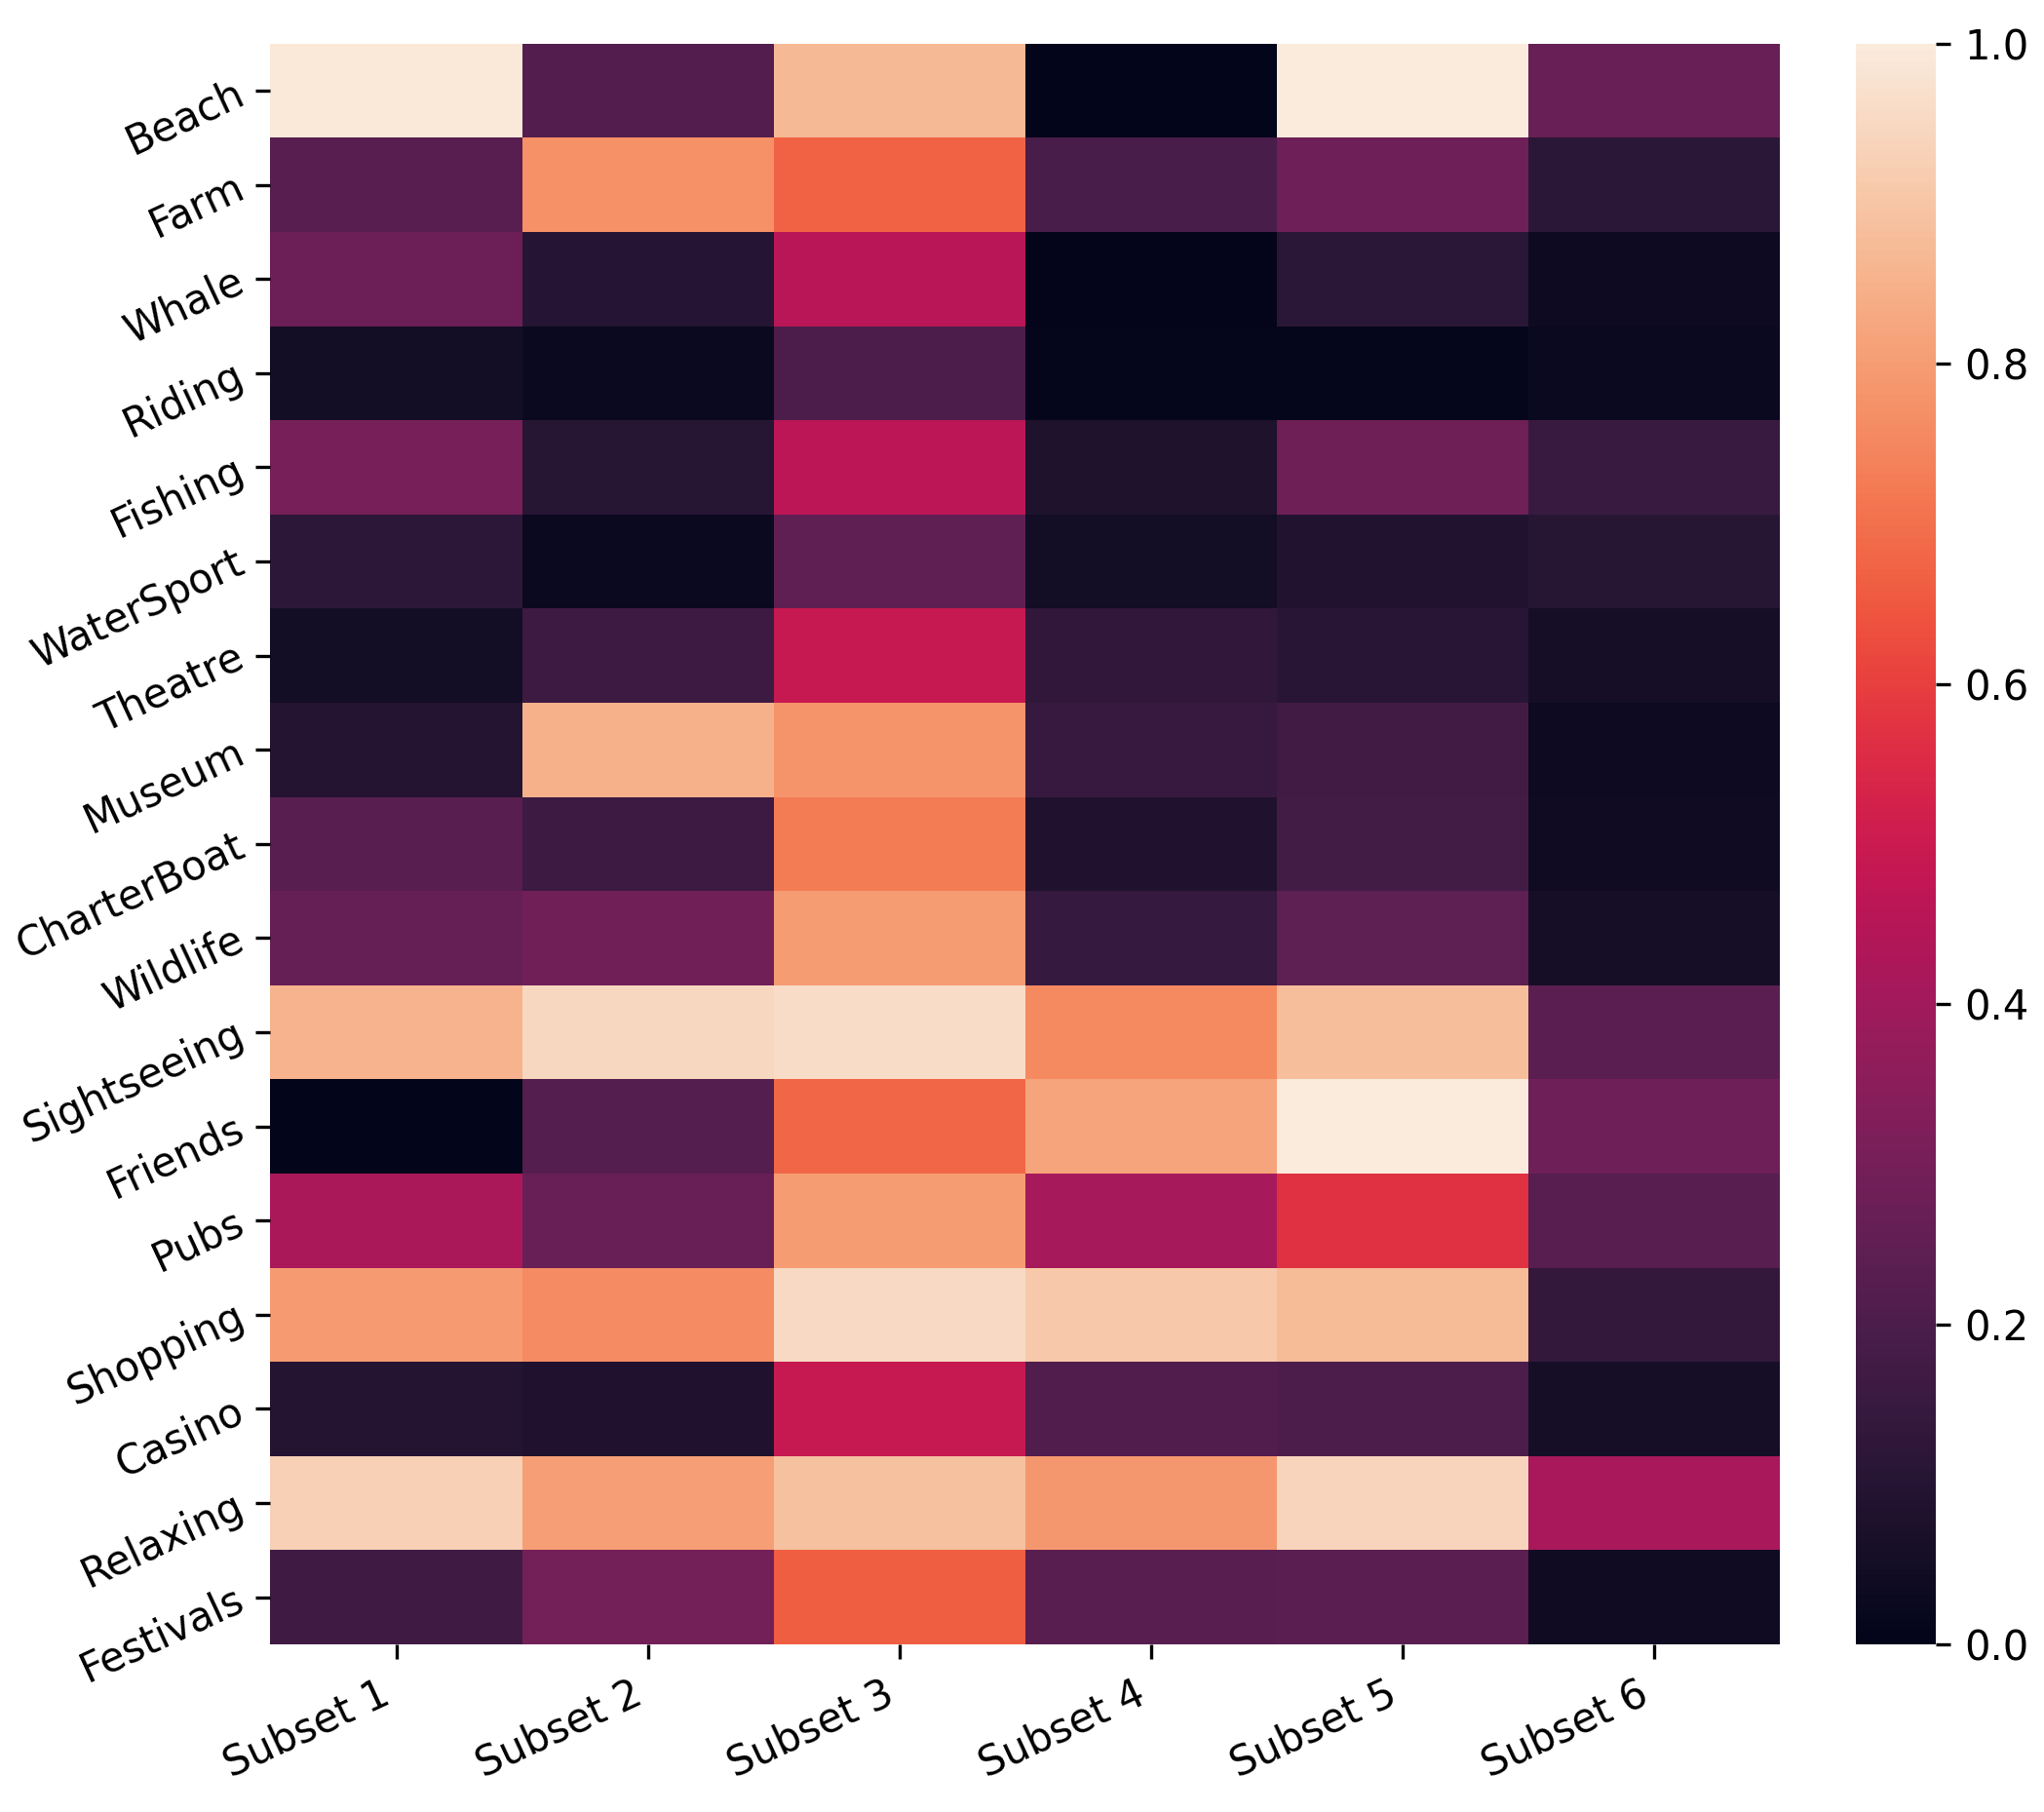
\includegraphics[width=1\textwidth]{aus_heatmap.png}
    \caption{Heatmap of the intra cluster fraction (indicated by color) of the k-means solution with \( k = 6 \) and the reduced feature subset. We can observe that tourists in subsets 1, 2 and 6 all prefer to travel without their friends.}
    \label{fig:aus_heatmapg}
\end{figure}

\begin{figure}[h!]
    \centering
    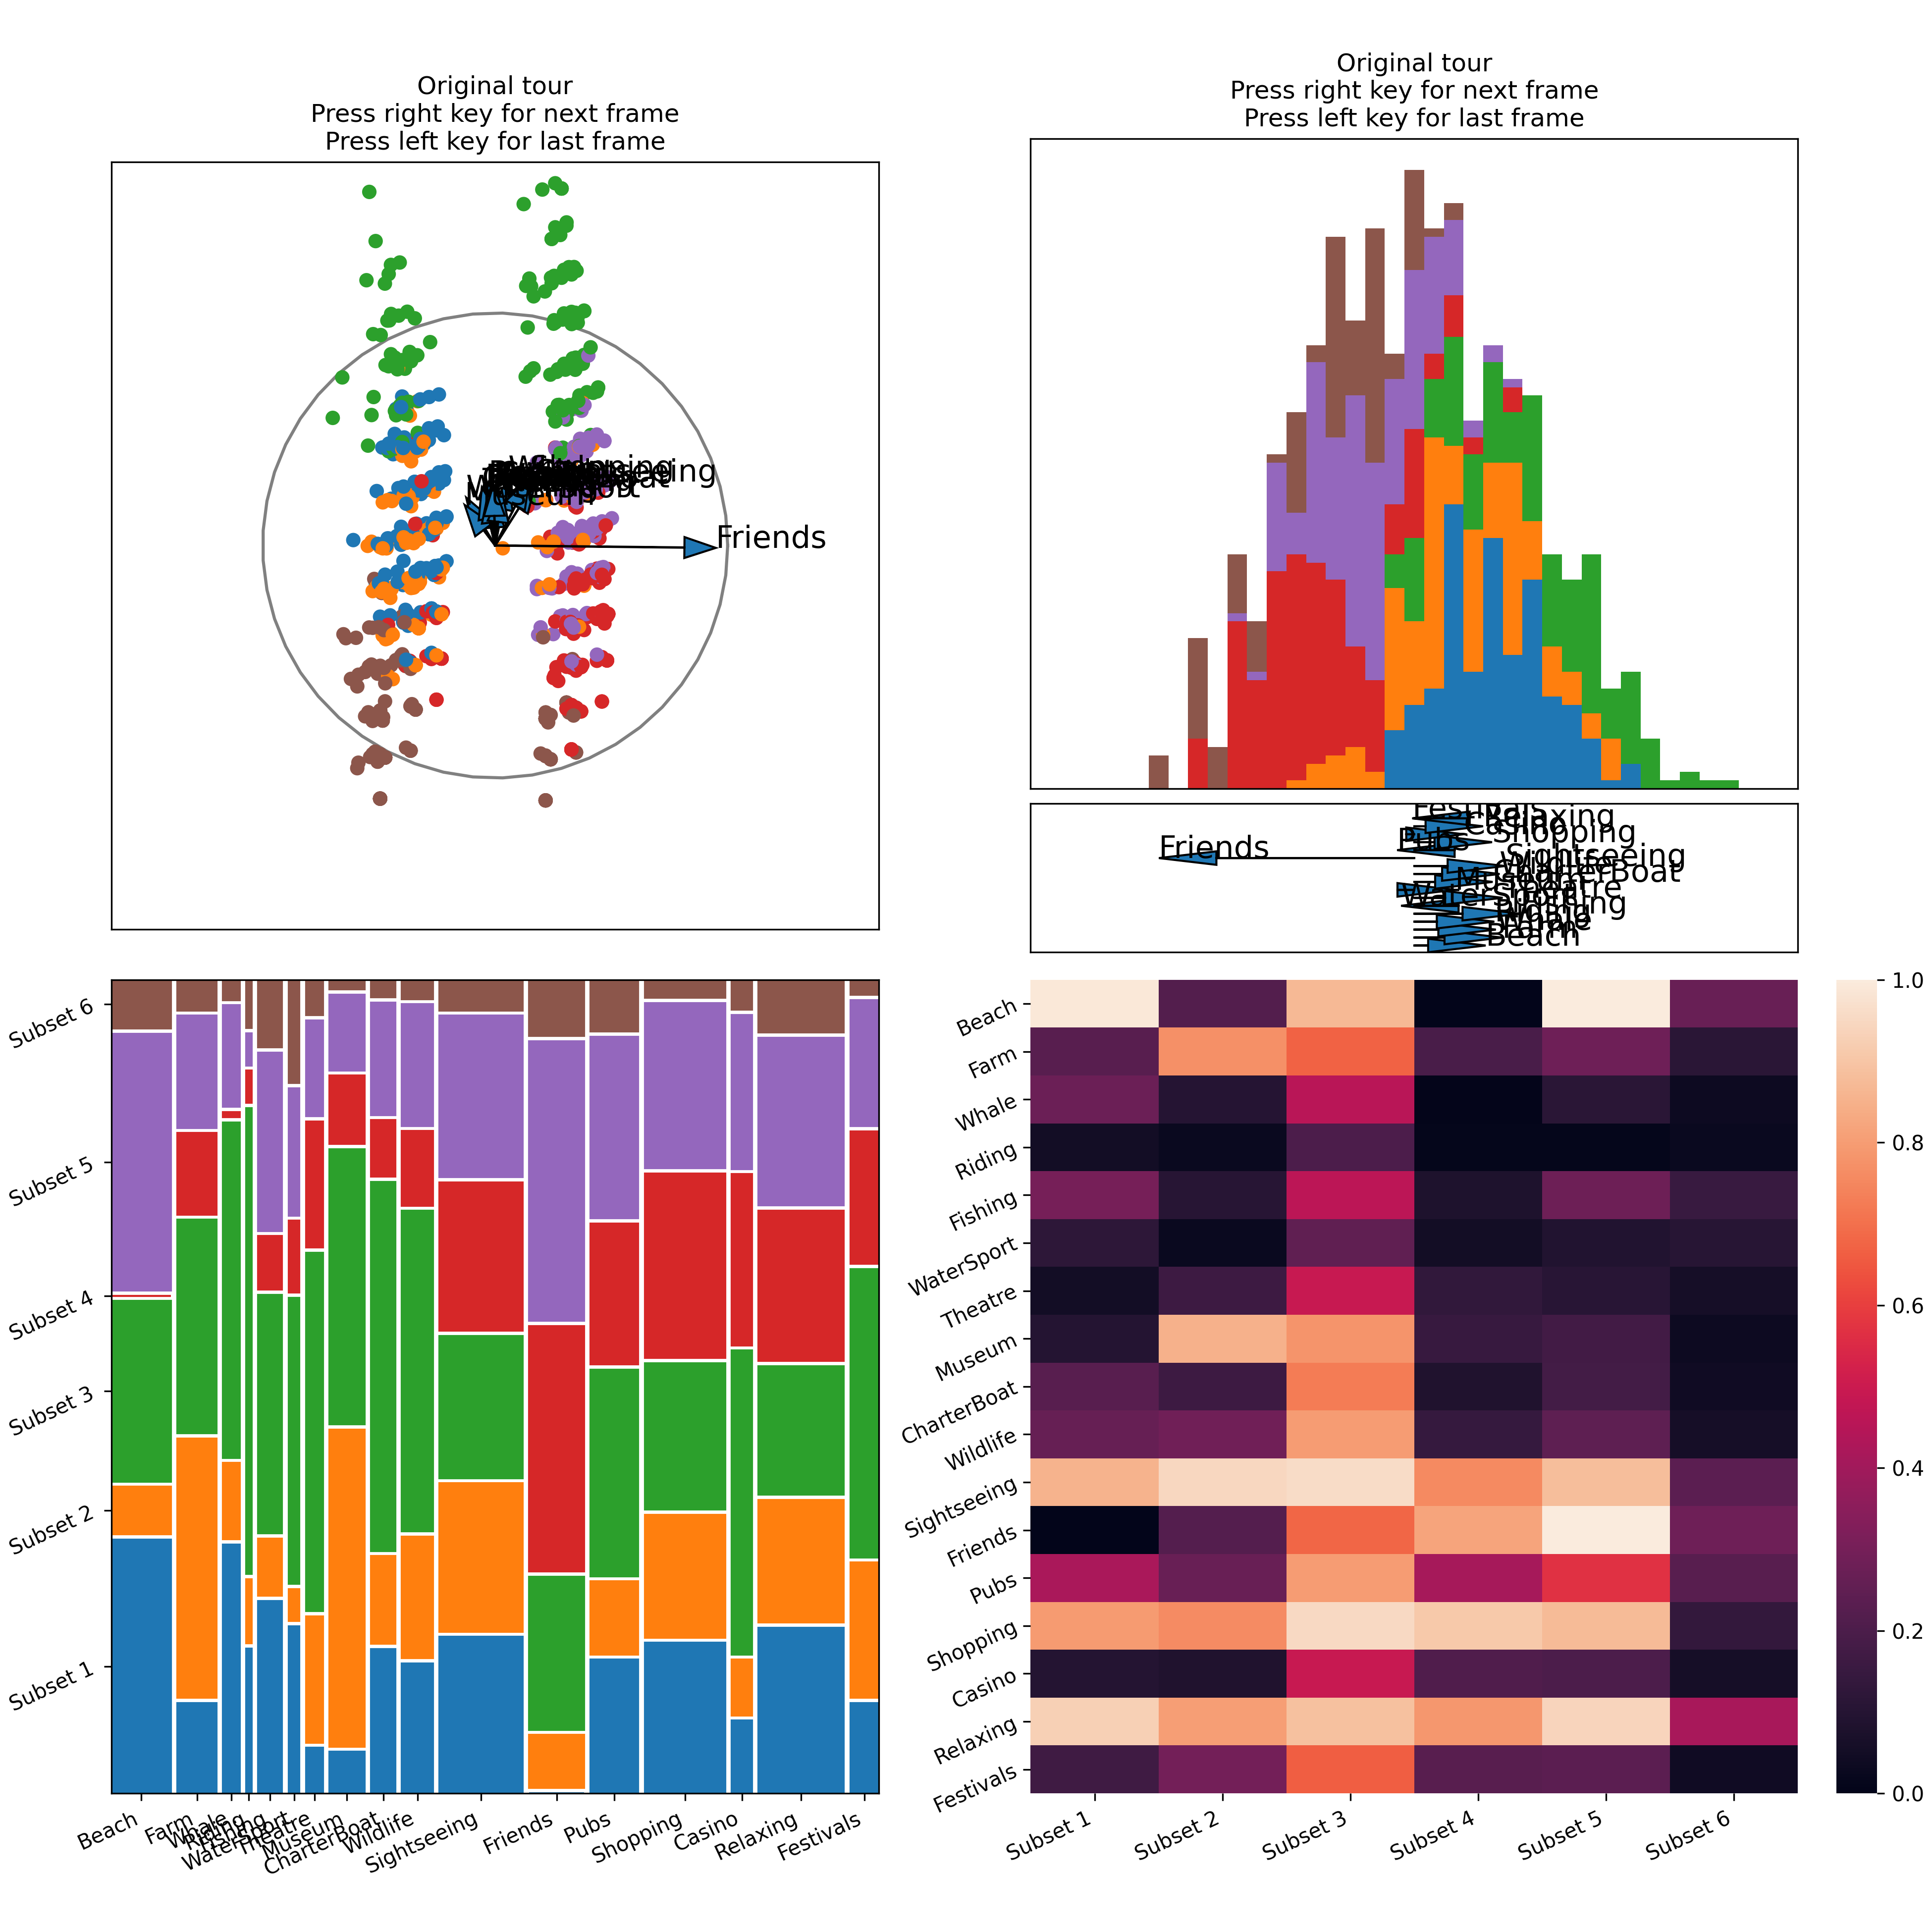
\includegraphics[width=1\textwidth]{aus_preselection.png}
    \caption{Interactive tour GUI loaded with multiple plots showing different aspects of the k-means solution of the Australian vacation activities dataset, with the projection axes of the feature ``Friends'' pointing into one direction and all the other ones into another one. Top left: 2D tour. Top right: 1D tour. Bottom left: Mosaic plot. Bottom right: Heatmap with the intra cluster fraction. We can see how the feature ``Friends'' and the general activity level (represented by the other projection axes pointing into one direction) separates the data.}
    \label{fig:aus_preselection}
\end{figure}


\begin{figure}[h!]
    \centering
    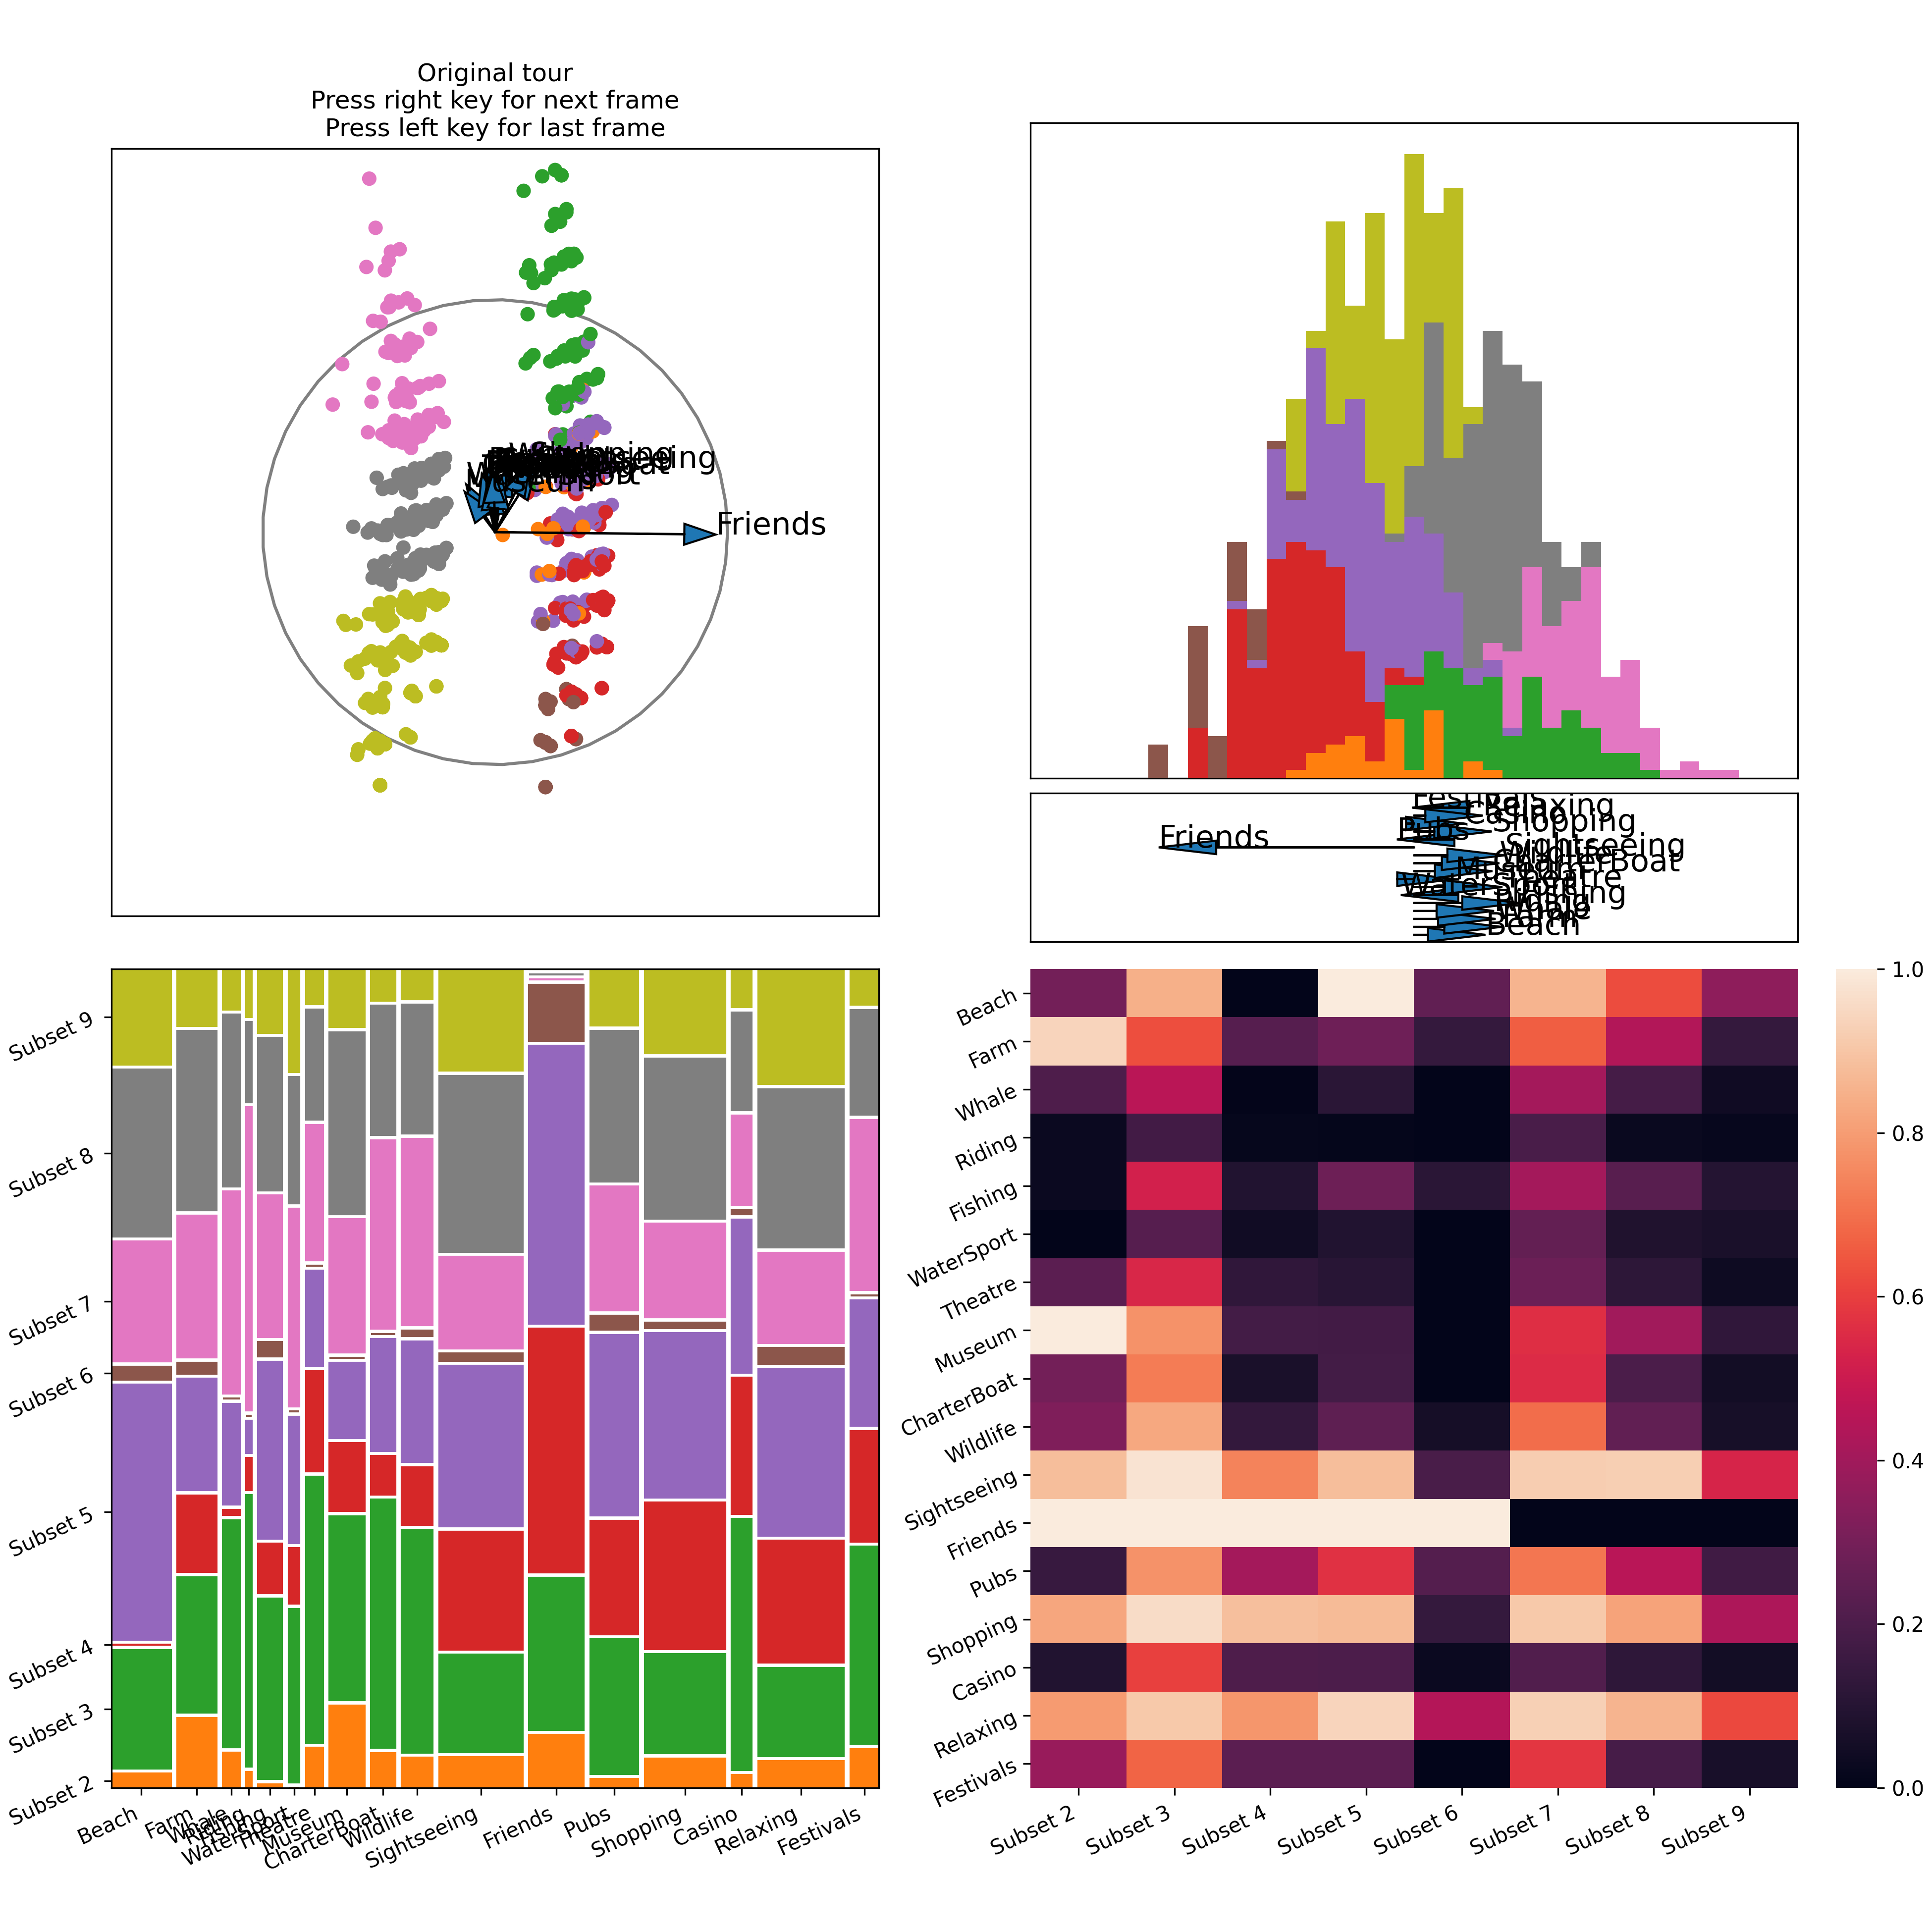
\includegraphics[width=1\textwidth]{aus_selection.png}
    \caption{Interactive tour GUI as seen in \ref{fig:aus_preselection}, but after sub-selection of subsets 7 (pink), 8 (grey) and 9 (gold). Top left: 2D tour. Top right: 1D tour. Bottom left: Mosaic plot. Bottom right: Heatmap with the intra cluster fraction. We can observe the preferences of three new subsegments, which can be interpreted as very active (pink), moderately active (grey) and inactive (gold) tourists travelling without their friends.}
    \label{fig:aus_selection}
\end{figure}


\section{Discussion}~\label{discussion}

One might question the necessity of manual exploratory data analysis, considering it is inherently subjective and relies heavily on intuition. However, in situations like those presented here, where there is no clearly defined or optimal clustering solution or feature selection, manual exploration becomes indispensable. While it is possible to optimize clustering metrics to improve separation between clusters, this alone may not yield conclusions that are useful for practical applications. The lack of clear boundaries and the overlapping nature of clusters in the datasets underscore the limitations of purely automated methods in capturing the complexity and nuance of real-world data.

In such cases, manual exploration allows analysts to interweave expert knowledge, intuition, and specific objectives with the initial clustering solution, which serves as the backbone of the analysis. This approach is particularly valuable when no single solution can be deemed “correct.” For instance, in the Austrian dataset, leveraging the interactive GUI for feature selection enabled us to isolate the most informative activities and gain deeper insights into the preferences of tourists who might be interested in visiting museums. This understanding facilitated targeted recommendations for increasing museum attendance by focusing on tourists frequenting hiking trails, excursion spots, and shopping centers. Such insights are challenging to extract through automated optimization alone.

Similarly, in the Australian dataset, manual exploration allowed us to refine the understanding of solo travellers by dividing them into three distinct subsegments: highly active, moderately active, and largely inactive tourists. This nuanced segmentation, derived from a blend of automated clustering and manual adjustments, offers a deeper understanding of the varied needs and behaviors within this group, enabling more effective marketing strategies.

While some plots supported by the pytourr package are specifically designed for analyzing binary survey data, it is important to emphasize that its capabilities extend far beyond this data type. The versatility of tours has been demonstrated across various applications in the past, showcasing their effectiveness in exploring complex, high-dimensional datasets. The interactive GUI enables seamless exploration of both one- and two-dimensional tours, regardless of the data being analyzed, providing a powerful tool for uncovering patterns and insights across diverse domains.


\section{Conclusion}~\label{conclusion}

Ultimately, manual data exploration serves as a useful complement to automated methods, providing the flexibility to incorporate context, expert judgment, and specific analytical goals. This approach enables analysts to refine initial results and adapt them to the complexities of real-world scenarios, leading to more nuanced interpretations and actionable insights. The pytourr package offers an organised and responsive interactive tool for conducting such analyses, bridging the gap between automated clustering and exploration.

By integrating interactive visualization capabilities, the pytourr package empowers users to dynamically engage with their data, making it possible to uncover subtle patterns and relationships that might otherwise remain hidden. This is especially valuable in tackling complex datasets with the mindset that an automated solution needs to be validated. The package has broad applicability across various data types and analytical contexts where clustering is used. The flexibility of setting up the GUI elements from the command line allow it to be tailored for different applications.

Future developments in the software might include expanding the range of interactive features and providing additional visualization methods.  Because it is built on R and python, it would also be possible to integrate more closely with the machine learning algorithms, such as generating new cluster solutions directly from the GUI. For more complex shapes, containing concavities, or non-linear boundaries, implementation of sliced tours~\citep{Laa2020}, would be recommended.

In summary, pytourr represents a significant advancement in the toolkit of data analysts, offering a novel way to balance automated analysis with human intuition and domain expertise, thereby facilitating a deeper and more comprehensive understanding of complex datasets.


%\bibliographystyle{plainat}
\bibliography{pytourr_references.bib}



\end{document}
